%% main_ppgco_ufu.tex v1.0, Lásaro Camargos e Denise Guliato
% adaptado de modeloABNT2.tex, v1.0 athila
% ------------------------------------------------------------------------
% ------------------------------------------------------------------------
% eesc: Modelo de Trabalho Acadêmico (tese de doutorado, dissertação de
% mestrado e trabalhos monográficos em geral) em conformidade com 
% ABNT NBR 14724:2011. Esta classe estende as funcionalidades da classe
% abnTeX2 elaborada de forma a adequar os parâmetros exigidos pelas 
% normas USP e do departamento de elétrica da Escola de Engenharia 
% de São Carlos - USP.
% ------------------------------------------------------------------------
% ------------------------------------------------------------------------
% Atualizações.
% 07/05/2015 - adicionada a seção de atualizações neste template.
% 18/11/2015 - atualizações para dissertações e teses com corpo em inglês
% 19/01/2021 - alterações nas referências com >3 autores (agora mostra todos)/
%              impressão de um lado somente
%              lista de algoritmos e lista de códigos
% ------------------------------------------------------------------------
% Opções:
% tesedr:     Formata documento para tese de doutorado
% qualidr:    Formata documento para qualificação de doutorado
% dissertmst: Formata documento para dissertação de mestrado
% qualimst:   Formata documento para qualificação de mestrado
% ------------------------------------------------------------------------
\documentclass[dissertmst]{ppgco}
%Não altere o comando seguinte. O título de seu trabalho será especificado mais adiante.
\title{Template de Monografia do PPGCO}

% ---
% PACOTES
% ---

% ---
% Pacotes fundamentais 
% ---
%\usepackage{cmap}				% Mapear caracteres especiais no PDF
\usepackage{graphicx,url}
\usepackage[brazil]{babel}
\usepackage[utf8]{inputenc}
\usepackage{mdframed}
\usepackage{float}
\usepackage{amsmath}
\usepackage{pdflscape}
\usepackage{fancybox}
\usepackage{pdfpages}
\usepackage{subcaption}
% ---

% ---
% Pacotes adicionais, usados apenas no âmbito do Modelo eesc
% ---
\usepackage[printonlyused]{acronym}

% ---


% ---
% Informações de dados para CAPA e FOLHA DE ROSTO
% ---
%
% Título:
%	1. Título em português
%	2. Título em inglês
\titulo{Segmentação Automática de Canais Vasculares em Imagens Histológicas de Tecido Ósseo Utilizando Redes Neurais Completamente Convolucionais}

%
% Autor:
%	1. Nome completo do autor
%	2. Formato de nome para bibliografia
\autor{Igor Gonçalves Ribeiro Silva}{Silva, Igor}
%
% Cidade
\local{Uberlândia}
% Ano de defesa
\data{2024}
% Área de concentração da pesquisa
\areaconcentracao{Ciência da Computação}
% Nome do orientador
\orientador{Bruno Augusto Nassif Travençolo}
% Nome do coorientador
%\coorientador{Nome completo do coorientador}
% ---

% ---
% compila o indice
% ---
\makeindex
% ---

% ---
% Compila a lista de abreviaturas e siglas
% ---
\makenomenclature
% ---

% ---
% Inserir ficha catalográfica
%
% Caso o comando \inserirfichacatalografica seja definido, a %ficha catalográfica
% será inserida atrás da folha de rosto. Caso contrário a página será deixada em
% branco.
%
% CUIDADO: Esta opção deve ser preenchida antes do comando \maketitle
% ---
%entre em contato com a biblioteca para obter a sua ficha catalográfica em arquivo pdf. Essa %folha só será inserida no documento após a sua defesa.

%\inserirfichacatalografica{fichaCatalografica.pdf}
% ---

% ----
% Início do documento
% ----

\begin{document}

% elementos pré-textuais ainda estão em inglês no template, voltando para ptbr
\renewcommand{\orientadorname}{Orientador: }
%\renewcommand{\coorientadorname}{Coorientador: }
\renewcommand{\agradecimentosname}{Agradecimentos}

% ----------------------------------------------------------
% ELEMENTOS PRÉ-TEXTUAIS
% ----------------------------------------------------------
\pretextual

% ---
% Insere Capa, Folha de rosto, Ficha catalográfica (se inserida)
% e folha de aprovação (se inserida).
% ---
\maketitle


% ---
% Dedicatória
% ---
%\imprimirdedicatoria{Escrever dedicatória}
% ---

% ---
% Agradecimentos
% ---
\imprimiragradecimentos{
Agradeço à Universidade Federal de Uberlândia, em especial a Faculdade de Computação, todo o seu corpo docente, direção e administração por esta oportunidade de crescimento pessoal, profissional e acadêmico.

Ao meu orientador Bruno Augusto Nassif Travençolo por todo o suporte e incentivo e compreensão presentes nas incontáveis aulas e reuniões e todas as suas correções e ensinamentos que muito contribuíram para minha formação como pessoa e pesquisador.

À professora Paula Dechichi pela disponibilização do material biológico utilizado no desenvolvimento do trabalho, bem como o incentivo e apoio para o desenvolvimento dele. 

A minha esposa Camila que, além da participação ativa no desenvolvimento deste trabalho, pelo incentivo em retornar à academia e todo o apoio, amor e compreensão durante esse período. Sem ela, por diversos motivos, este trabalho não seria realizado.

A minha mãe Maria de Fátima, que nunca mediu esforços nem incentivos para que eu pudesse construir uma vida digna através dos estudos.

A minha tia Geralda Gislene deu todo o apoio e carinho durante minha graduação, tornando possível tal importante passo em minha carreira.

}
% ---

% ---
% Epígrafe
% ---
%\imprimirepigrafe{
%		``Sua vida pode ser dividida em dois períodos: antes de agora e a partir de agora.''\\
%		(Prof. Obvious Stating)
%}
% ---

% ---
% RESUMO e ABSTRACT
% ---

% Resumo em português - as palavras entre chaves são as palavras-chave do trbalho

\begin{resumo}{Segmentação de imagens. Canais Ósseos. Redes Neurais Convolucionais}

Neste trabalho é proposto um método de segmentação de canais ósseos em imagens histológicas de lâmina inteira. O método faz uso de uma rede neural originalmente desenvolvida com o intuito de segmentar tumores derivados da cavidade oral em imagens histológicas coradas com Hematoxilina e Eosina, e foi adaptado para o contexto de canais ósseos. O conjunto de dados é composto por 65 imagens de lâmina inteira, as quais foram coradas com Hematoxilina e Eosina e extraídas a partir do fêmur de ratos saudáveis da linhagem Wistar.
Com a ajuda de um especialista em histologia, as imagens foram analisadas e seus canais ósseos foram manualmente marcados gerando um conjunto de máscaras binárias. As imagens de ambos os conjuntos (imagens originais e binárias) foram então divididas em sub-imagens de 640x640 pixels de tamanho. A rede foi treinada e validada com 1722 sub-imagens. O treinamento contou ainda com uma estratégia de aumento de dados com sete possíveis variações das imagens. O método foi avaliado comparando-se as regiões segmentadas pela rede com as marcações do especialista. Foram calculadas a acurácia, especificidade, sensibilidade, precisão, Intersecção sobre União e \textit{f1-score} das segmentações resultantes. Além disso, foi feita uma comparação com outro método de segmentação automática de canais ósseos encontrada na literatura. O método validado por este trabalho mostrou-se eficiente e superior ao método com o qual foi comparado, apresentando \textit{f1-score} de 84,9\% e Intersecção sobre União de 73,7\%, além de bons resultados qualitativos.

\end{resumo}


% Resumo em inglês
\begin{abstract}{Image Segmentation. Bone Canals. Convolutional Neural Networks}

This study proposes to validate a method that use fully convolutional neural networks for segmentation of bone canals on whole slide images. A neural network developed originally for segmenting tumors derived from the oral cavity in histological images stained with Hematoxylin and Eosin was used. The dataset was composed by 65 whole slide images images extracted from the femur of healthy Wistar rats. With the help of a histology expert, 65 whole slide images images were analyzed and their bone canals were manually labeled. These images were preprocessed in order to generate binary images highlighting the region of interest and discarding the background. Then the images of both sets (original and binary images) were broken into patches of 640x640 pixels. The network was trained and validated with 1722 patches. During the training a data augmentation strategy was used with 7 possible variations of the images. The method was evaluated by comparing the regions segmented by the network with the manual labels. The accuracy, specificity, precision, sensitivity, Intersection over Union and f1-score of the resulting segmented images were calculated. Furthermore, the method was compared with another method for automatic segmentation of bone canals found in the literature. The method proved to be efficient and superior to the method that was compared with, reaching a f1-score close of 84,9\% and Intersection over Union of 73,7\%.
	
\end{abstract}

% ---

% ---
% inserir lista de ilustrações
% ---
\listailustracoes
% ---

% ---
% inserir lista de tabelas
% ---
\listatabelas
% ---

% ---
% inserir lista de códigos (específicos de linguagens)
% ---
%\listadecodigos

% ---
% inserir lista de algortimos (pseudocódigos)
% ---
%\listadealgoritmos

% ---
% inserir lista de abreviaturas e siglas
% ---
\listasiglas{abrev/Abreviaturas}
% ---

% ---
% inserir o sumario
% ---
\sumario
% ---

% ----------------------------------------------------------
% ELEMENTOS TEXTUAIS
% ----------------------------------------------------------
\mainmatter


% ----------------------------------------------------------
% Copyright
% ----------------------------------------------------------
%\newpage
%\thispagestyle{empty}

%\ \

%\vspace{10cm}

%I hereby certify that I have obtained all legal permissions from the owner(s) of each third-party copyrighted matter included in my dissertation, and that their permissions allow availability such as being deposited in public digital libraries.

%\vspace{5cm}

%\begin{center}
%Igor Gonçalves Ribeiro Silva
%\end{center}


% ----------------------------------------------------------
% Introdução
% ----------------------------------------------------------
\chapter[Introdução]{Introdução}

A histologia é a área da biologia que estuda tecidos e composição de órgãos. Ela possui grande relevância na área acadêmica pois tem como proposta estudar a estrutura e a função dos tecidos, realizar análises quantitativas, avaliar respostas a tratamentos e investigar aspectos do desenvolvimento embrionário e da fisiologia. Outras aplicações importantes da histologia são encontradas na medicina, em que é empregada em diagnósticos médicos, auxiliando patologistas a identificar e caracterizar doenças, tumores, infecções e outras alterações nos tecidos~\cite{junqueira1985histologia}. 

As análises histológicas são comumente feitas a partir de imagens denominadas cortes histológicos, que podem ser obtidas em laboratório por meio de um longo processo de preparo. A análise desses imagens de lâmina inteira muitas vezes são demoradas e demandam grande esforço de um especialista ~\cite{linhares2022automated}. Dada a importância da análise histológica, é interessante desenvolver métodos que possam facilitá-la, tornando-a mais rápida e acessível para os pesquisadores e profissionais da saúde.

 O tecido ósseo é um tecido conjuntivo que tem grande relevância em pesquisas da área da histologia devido à sua estrutura, composição e propriedades regenerativas. Desenvolver formas de automatizar a análise de imagens histológicas de tecido ósseo pode auxiliar estudos relacionados à estrutura do tecido, sua regeneração e efeitos de tratamentos de doenças ~\cite{linhares2019melhoria}. Porém é um desafio automatizar tais análises devido a vários fatores como o tamanho das imagens, complexidade e quantidade de estruturas, irregularidades e rasgos no tecido decorrentes do processo de preparo do corte histológico \cite{gondim2021automatic}.


Nos últimos anos o aprendizado de máquina tem ganhado destaque tanto no meio acadêmico como no corporativo por apresentar resultados satisfatórios na execução de tarefas complexas, inclusive em relação ao processamento de imagens~\cite{miklosik2020impact}. Uma das abordagens do aprendizado de máquina é o aprendizado supervisionado, cujo princípio é o uso de uma base de dados para treinar um modelo de forma que o mesmo aprenda a realizar uma determinada tarefa. Esse conjunto de dados deve estar organizado de forma a conter exemplos diversos de entradas de dados e suas respectivas saídas esperadas~\cite{monard2003conceitos}. 
    
    Entretanto, ao se trabalhar com modelos de aprendizado de máquina, o conjunto de dados a ser utilizado pode ser um fator limitante, pois é preciso um conjunto de dados bem estruturado para se realizar a tarefa desejada a fim de se realizar um treinamento que não seja enviesado e que apresente bons resultados~\cite{paullada2021data}. Dessa forma, para se criar e treinar um modelo de aprendizado de máquina para a execução de uma tarefa, muitas vezes é necessário um árduo trabalho prévio de elaboração de um conjunto de dados que viabilize o treinamento.
    
    Conjuntos de imagens são amplamente utilizados em técnicas de aprendizado profundo (do inglês \textit{deep learning}), uma subárea do aprendizado de máquina. O uso de redes neurais, modelos de aprendizado de máquina que tentam simular estruturas do cérebro humano, tem apresentado resultados interessantes no campo da visão computacional, especialmente as \acf{RNC}. Tais redes se baseiam na forma como os seres humanos percebem e aprendem características chave das imagens~\cite{rawat2017deep}.
    
    O uso do aprendizado profundo na área médica vêm ganhando força e importância especialmente desde o surgimento das redes do tipo U-Net, arquitetura proposta em 2015 por \cite{ronneberger2015u} que vem sido amplamente utilizada para segmentação de imagens biomédicas graças à sua capacidade de realizar classificação a nível de pixel. A utilização de tais técnicas pode ser de grande ajuda para especialistas em análises clínicas, diagnósticos e pesquisas, tornando o processo mais acessível e ágil~\cite{esteva2021deep}.

\section{Motivação}

Sabendo da importância da visão computacional nas ciências biomédicas, e do importante papel que o aprendizado profundo vem desempenhando na área de visão computacional, é interessante oferecer ferramentas que façam algum tipo de processamento automático em imagens histológicas, tais como classificação de imagens ou segmentação semântica. 
    
    Existem alguns métodos que visam resolver problemas específicos no processamento automático de imagens, como segmentação de alguma estrutura específica a partir da aplicação de determinados procedimentos nas imagens, como o proposto em~\cite{gondim2021automatic}. Porém tais métodos muitas vezes não apresentam invariância, ou seja, não costumam reagir bem a variações nas entradas, como tamanho das imagens, ruídos, variações de cor e posicionamento. Isso dificulta a utilização dessas ferramentas, visto que a parametrização ideal pode ser diferente para cada entrada~\cite{linhares2022automated}, o que levou ao questionamento sobre a possibilidade de se criar uma ferramenta de processamento de imagens que possa se ajustar automaticamente para a realização de uma determinada tarefa independentemente das características específicas de cada imagem a ser analisada.
    
    Para a realização desse tipo de trabalho, as \acs{RCN}s têm apresentado ótimos resultados, pois por meio da convolução aprendem padrões de imagens em um nível local e os identificam na imagem independente de posição, tamanho ou rotação~\cite{mueller2019deep}. Portanto deve ser possível utilizar uma \acs{RCN} que realize segmentação de estruturas de interesse em imagens histológicas de tecido ósseo com desempenho e precisão satisfatórias.
    
    Entretanto, como já mencionado, utilizar uma rede neural para este tipo de tarefa requer um conjunto de dados estruturado de forma adequada.
    Existem vários conjuntos de dados de imagens médicas disponíveis para uso, por exemplo o ALL-IDB \cite{Labati2011} e ErythrocytesIDB \cite{Gonzalez-Hidalgo2015}, que são conjuntos de amostras de sangue; e o COVID-19 Radiography Database \cite{Chowdhury2020}, conjunto de imagens de raio-x de pulmões de pacientes com COVID-19. Porém observou-se uma escassez de dados destinado especificamente à segmentação de imagens histológicas de tecido ósseo.
    
\section{Objetivo}

    Partindo da ideia apresentada, o objetivo deste trabalho é validar o uso de uma \ac{RNC} como método de segmentação de canais vasculares em imagens histológicas de tecido ósseo. O método testado deve alcançar resultados aceitáveis e comparáveis com métodos já existentes.
    
    Um desafio deste trabalho é a preparação do \textit{dataset}, que será feito por meio da marcação da região de interesse em várias imagens de lâmina inteira. Tais marcações serão realizadas com a ajuda de um especialista em histologia.

\section{Hipótese}
Este trabalho busca validar a seguinte hipótese: \bigskip

\setlength{\fboxsep}{12pt}
\shadowbox{\parbox{0.89\textwidth}{
\textit{É possível utilizar Redes Neurais Convolucionais para realizar a segmentação de canais ósseos em imagens histológicas com precisão aceitável em relação à posição e à forma das estruturas em questão.}
}}
\bigskip

\section{Contribuições}

    A principal contribuição esperada deste trabalho é demonstrar a viabilidade do uso de Redes Neurais Convolucionais para a tarefa de segmentação de canais ósseos em imagens histológicas, abrindo assim portas para o uso de \ac{RNC}s em outras tarefas da histologia relacionadas a imagens de tecido ósseo e para o desenvolvimento de novas tecnologias que possam contribuir para pesquisas dessa área.
    
Outra contribuição é a disponibilização pública de um conjunto de imagens histológicas de tecido ósseo, que pode vir a ser útil para outros pesquisadores na elaboração e desenvolvimento de suas pesquisas. Tal conjunto pode ser evoluído em trabalhos posteriores para que seja possível realizar outras tarefas de visão computacional em imagens de tecido ósseo, como classificação ou segmentação de outras estruturas presentes nesse tipo de tecido.  


% ----------------------------------------------------------
% Fundamentação
% ----------------------------------------------------------
\chapter[Fundamentação Teórica]{Fundamentação Teórica}

Neste capítulo são abordados os conceitos fundamentais que embasam o desenvolvimento desta pesquisa e os principais trabalhos correlatos.

\section{O tecido ósseo e a rede vascular}
O tecido ósseo é um dos objetos de estudo da histologia e chama a atenção de pesquisadores e profissionais da área médica especialmente devido às suas propriedades regenerativas. Macroscopicamente os ossos longos podem ser divididos em duas regiões: diáfise e epífise. As epífises são as extremidades do osso e são compostas por osso esponjoso, ou seja, com muitas cavidades intercomunicantes \cite{junqueira1985histologia}. Já a diáfise é a região intermediária do osso, sendo mais fina e apresentando osso compacto -- sem cavidades -- em sua maior parte~\cite{junqueira1985histologia}. A Figura~\ref{fig:estrutura-ossos-longos}(a) mostra tais regiões e suas respectivas composições.

A maior parte da diáfise é composta túneis longitudinais formados por lamelas concêntricas, tais túneis são conhecidos como sistema de Havers e formam em seus centros canais que são percorridos por vasos sanguíneos, linfáticos e nervos. Também existem canais transversais que conectam canais de Havers adjacentes chamados canais de Volkmann, formando assim a rede de canais ósseos~\cite{junqueira1985histologia}. A Figura~\ref{fig:estrutura-ossos-longos}(b) ilustra as estruturas mencionadas destacando os canais de Havers e de Volkmann.

\begin{figure}[H]
    \centering
    \center
    \begin{tabular}{@{}c@{}}
        \includegraphics[width=.4\linewidth]{figures/2_theoric_foundamentations/estruturaosso.png}
        \\[\abovecaptionskip]
        \small (a)
    \end{tabular}
    \begin{tabular}{@{}c@{}}
        \includegraphics[width=.4\linewidth]{figures/2_theoric_foundamentations/sistemahavers.png}
        \\[\abovecaptionskip]
        \small (b)
    \end{tabular}
  
    \caption[Estrutura básica de um osso longo.]{Estrutura básica de um osso longo. Em (a) os principais componentes anatômicos de um osso longo. Em (b) os canais de Havers e Volkmann, que compõem o osso compacto, principal componente da diáfise, região intermediária de ossos longos. Fonte: \cite{junqueira1985histologia}}
    \label{fig:estrutura-ossos-longos}
\end{figure}

Os vasos sanguíneos e linfáticos que percorrem os canais nutrem os osteócitos, que são estruturas que cumprem um importante papel na manutenção e integridade da matriz óssea. Dessa forma a rede de canais ósseos cumpre um importante papel de nutrição do tecido contribuindo para seu desenvolvimento e no processo de reparo ósseo \cite{junqueira1985histologia}.

A Figura~\ref{fig:corte-canais-osteocitos} ilustra um corte transversal na diáfise de um osso longo e um exemplo de imagem histológica dessa região, destacando os canais ósseos e os osteócitos.
\begin{figure}[H]
    \centering
    \center
    \begin{tabular}{@{}c@{}}
        \includegraphics[width=.8\linewidth]{figures/2_theoric_foundamentations/Corte-canais-osteocitos.png}
        \\[\abovecaptionskip]
    \end{tabular}
  
    \caption[Corte transversal da diáfise de um osso longo]{Corte transversal da diáfise de um osso longo com uma região ampliada destacando alguns canais ósseos e osteócitos.}
    \label{fig:corte-canais-osteocitos}
\end{figure}

\section{Aprendizado de máquina} \label{subsec:AutoML}
Ainda em 1959 Arthur Lee Samuel definiu o aprendizado de máquina como ``o campo de estudo que dá aos computadores a habilidade de aprender sem serem explicitamente programados''~\cite{simon2013too}. De fato o aprendizado de máquinas automatizado permite, por exemplo, que computadores aprendam a realizar tarefas analisando uma base de dados previamente rotulada, além de aprimorar seu aprendizado à medida que novos dados lhe são apresentados \cite{monard2003conceitos}.

O aprendizado de máquina é um área da inteligência artificial que se apoia em técnicas e conceitos da matemática e estatística. Esse aprendizado é dividido em quatro tipos: aprendizado supervisionado, não supervisionado, auto supervisionado e por reforço. Todos possuem uma variedades de algoritmos, sendo que, para cada problema a ser resolvido, um determinado algoritmo pode ser mais adequado que os demais \cite{mueller2019deep}.

Como mencionado acima, uma das técnicas de aprendizado de máquina é o aprendizado supervisionado. Nessa abordagem utiliza-se uma base de dados na qual para cada entrada o resultado desejado é conhecido. As entradas com seus respectivos resultados esperados, também chamados de rótulos, são apresentados ao algoritmo em uma etapa conhecida como etapa de treinamento, em que o algoritmo ajusta, com base nos dados fornecidos, uma série de parâmetros internos a fim de encontrar padrões que o permitam estimar resultados para novas entradas \cite{monard2003conceitos}. A saída pode ser qualitativa, tratando-se assim de uma tarefa de classificação; ou quantitativa, tratando-se assim de uma tarefa de regressão \cite{mueller2019deep}.

\section{Aprendizado Profundo}

Uma subárea do aprendizado de máquina é o aprendizado profundo, que também trabalha com grandes conjuntos de dados para aprender a realizar tarefas. A grande diferença é que, ao invés de métodos e modelos estatísticos, o aprendizado profundo faz uso de apenas uma técnica que simula o funcionamento do cérebro humano: as redes neurais \cite{mueller2019deep}. 

Redes neurais podem possuir diversas camadas e arquiteturas, sendo que cada uma pode ser mais ou menos indicada para cada tipo de problema a ser tratado.
Tais redes são compostas por estruturas chamadas neurônios, que simulam os neurônios biológicos e se ligam uns aos outros por meio de ligações com diferentes pesos que simulam as sinapses cerebrais \cite{mueller2019deep}.

A rede neural mais simples possível é o \textit{perceptron}, que pode ser utilizada para tarefas de classificação binária ou regressão linear. O \textit{perceptron} é composto por apenas uma camada de um único neurônio. Ele recebe uma entrada $X$ de tamanho $m$ que é multiplicada por um vetor de pesos $W$ também de tamanho $m$. Em seguida é aplicada sobre o produto escalar $X \cdot W$ uma função de ativação a fim de produzir um único resultado de saída \cite{block1962perceptron}. O processo de treinamento de uma rede neural consiste justamente em realizar, com base no conjunto de dados de entrada, a parametrização do vetor de pesos $W$ das ligações entre os componentes da entrada $X$ e o neurônio \cite{mueller2019deep}.

A partir do \textit{perceptron}, novas arquiteturas de redes neurais podem ser formuladas adicionando mais camadas, mais neurônios, funções de retro-propagação de erro dentre outras estratégias que permitem que as redes neurais resolvam problemas mais complexos.

\section{Redes Neurais Convolucionais}

Desde o ano de 2012, quando a arquitetura \textit{AlexNet} venceu a competição \textit{ImageNet Large Scale Visual Recognition Challenge (ILSVRC)}, as \acf{RNC} vêm ganhando popularidade na execução de tarefas relacionadas a processamento de imagens, vídeos e até mesmo voz \cite{vargas2016estudo}.
Esse tipo de rede neural é uma variação das redes de \textit{perceptron} multicamada, e se baseia no princípio biológico da percepção visual dos seres humanos a fim de minimizar o processamento dos dados para obter o resultado esperado \cite{mueller2019deep}. São compostas por camadas convolucionais, de agrupamento, achatamento e conectada. As próximas subseções detalham o papel de cada um desses elementos.

\begin{figure}[H]
  \centering
  \includegraphics[width=.8\linewidth]{figures/2_theoric_foundamentations/cnn.png}
  \caption[Estrutura básica de uma rede neural convolucional.]{Exemplo de estrutura básica de uma rede neural convolucional. Fonte: \cite{srinivasan2021durld}}
  \label{fig:cnn}
\end{figure}

\subsection{Camadas convolucionais}

Na arquitetura de uma \ac{RNC}, ilustrada na Figura \ref{fig:cnn}, ao receber uma imagem como entrada são utilizadas as ditas camadas convolucionais. Tais camadas aplicam filtros (também conhecidos por \textit{kernels}), representados por matrizes tridimensionais, sobre parte da imagem de entrada \cite{rawat2017deep}.

A aplicação desses filtros se dá por um algoritmo de janela deslizante, que percorre a imagem em seus três canais de cores utilizando um passo de determinado tamanho (também conhecido como \textit{stride}) realizando uma operação de produto escalar a fim de gerar uma nova matriz cujas dimensões podem ser menores ou iguais à anterior dependendo do tamanho do filtro e do \textit{stride}. As matrizes resultantes dessa operação entre os canais de cor e os filtros são chamadas de mapas de características, e suas dimensões variam de acordo com o tamanho do filtro (\textit{kernel}) e do passo da janela deslizante (\textit{stride}). Esses são importantes parâmetros que devem ser determinados durante o projeto da rede. Esse é o processo chamado convolução, que é ilustrado pela Figura \ref{fig:conv2d} e é o mais importante processo das \ac{RNC}s \cite{geron2019maos}. 


\begin{figure}[H]
  \centering
  \includegraphics[width=.5\linewidth]{figures/2_theoric_foundamentations/conv2d.png}
  \caption[Exemplo de convolução entre duas matrizes bidimensionais.]{Exemplo de convolução entre duas matrizes bidimensionais. O filtro K percorre a matriz I com um passo de uma unidade calculando os produtos escalares entre a respectiva região da matriz I e o filtro K, gerando assim uma nova matriz I*K que é o mapa de características, resultado da convolução entre I e K.}
  \label{fig:conv2d}
\end{figure}

\subsection{Camadas de agrupamento}

Após cada convolução é executada outra etapa importante do processamento em \ac{RNC}s que é o agrupamento. Para esta tarefa existem as camadas de agrupamento (do inglês \textit{pooling}) cuja função é diminuir o tamanho do mapa de características visando agilidade e invariância espacial \cite{rawat2017deep}. Essa etapa consiste na utilização de uma janela deslizante a qual é aplicada uma função que seleciona um único valor para representá-la, conforme ilustrado pela Figura \ref{fig:pooling}. O uso de funções de valor máximo, mínimo e médio é bastante comum nesta etapa \cite{geron2019maos}.

\begin{figure}[H]
  \centering
  \includegraphics[width=.5\linewidth]{figures/2_theoric_foundamentations/max_pooling_example.pdf}
  \caption[Agrupamento utilizando uma função de \textit{max-pooling}.]{Exemplo de agrupamento utilizando uma função de \textit{max-pooling}. O mapa de características é percorrido por uma janela deslizante que seleciona apenas o maior valor da região para compôr um mapa de caractrísticas menor.}
  \label{fig:pooling}
\end{figure}

Devido ao fato de diminuir o tamanho da imagem de entrada, essa etapa do processo -- composta por camadas de convolução seguidas de camadas de agrupamento -- também é conhecida como caminho de contração \cite{geron2019maos}.

\subsection{Camadas de achatamento}

Após as etapas de convolução é executada uma camada de achatamento (do inglês \textit{flatten layer}), na qual os mapas de características, que são matrizes, são transformados em um vetor que será usado para alimentar uma rede de neurônios multicamada. 

\subsection{Camada densa ou conectada}
A camada que comporta a rede de neurônios é chamada camada completamente conectada (ou densa) e tem por objetivo traçar a decisão a partir dos mapas de características. Esse tipo de camada é muito utilizado em tarefas de classificação \cite{rawat2017deep}.

Uma \ac{RNC} pode apresentar outros tipos de camadas além desses tipos básicos, ou ainda não apresentar alguma das camadas mencionadas acima dependendo do objetivo da rede \cite{mueller2019deep}.

\section{U-Net}
Proposta em 2015 por \cite{ronneberger2015u}, as redes U-Net vêm sendo aplicadas em diversos trabalhos referentes à segmentação de imagens médicas, uma vez que as redes de classificação, como as \ac{RNC}s tradicionais, não conseguem trazer informações contextuais a nível de pixel, o que é essencial em tarefas de segmentação, especialmente ao se trabalhar com imagens médicas \cite{siddique2021u}. 

As redes U-Net se diferem das \ac{RNC}s de classificação principalmente devido à adição de uma etapa de decodificação. Dessa forma, após passar pelo caminho de contração o vetor de saída é novamente transformado em uma matriz e esta é ampliada por algumas camadas de aumento até chegar ao tamanho original da entrada, sendo a imagem resultante uma máscara que representa a região de interesse segmentada. Esse processo também é conhecido como caminho de expansão. A combinação do caminho de contração com o caminho de expansão resulta em uma rede quase simétrica, cujo formato lembra a letra U, conforme ilustrado pela Figura \ref{fig:u-net-example}, dando assim o nome a esse tipo de rede \cite{ronneberger2015u}.

Outra interessante característica desse tipo de rede é a ausência de uma camada conectada, sendo que esta é substituída por camadas convolucionais que processam os mapas de características com mais eficiência que uma camada conectada, conforme descrito em \cite{long2015fully}. A ausência da camada conectada, dá o nome à arquitetura das \ac{RNCC}.

\begin{figure}
  \centering
  \includegraphics[width=.75\linewidth]{figures/2_theoric_foundamentations/u-net-example.png}
  \caption[Estrutura básica da rede U-Net.]{Estrutura básica da rede U-Net. Fonte: \cite{ronneberger2015u}}
  \label{fig:u-net-example}
\end{figure}

Assim, a arquitetura básica de uma U-Net, conforme foi originalmente proposta, consiste em um caminho de contração e um caminho de expansão. Durante a contração são aplicadas repetidamente duas convoluções com um filtro 3x3 seguidas de uma função de ativação \textit{ReLU} e um \textit{max-pooling} de tamanho 2x2, diminuindo em duas vezes e aumentando em duas vezes, respectivamente: o tamanho e o número dos mapas de características da saída da camada anterior \cite{siddique2021u}. 
Na expansão é feito o processo inverso: a cada camada é feito o aumento de resolução do mapa de características com uma convolução 2x2 que diminui pela metade os canais de características e dobra as dimensões da imagem (\textit{up-convolution}), uma concatenação com o mapa de características correspondente da etapa de contração e duas convoluções 3x3 seguidas por uma função de ativação \textit{ReLU}. Por fim é feita uma convolução 1x1 para mapear vetores de características para as classes desejadas. A rede possui um total de 23 convoluções \cite{ronneberger2015u}.

\section{Métricas de validação}
Esta seção apresenta e explica as principais métricas utilizadas para a validação do método proposto neste trabalho.
Para isso, consideremos a seguinte nomenclatura:

 \begin{itemize}
   \item VP - Verdadeiros positivos
   \item VN - Verdadeiros negativos
   \item FP - Falsos positivos
   \item FN - Falsos negativos
 \end{itemize}
   
\subsection{Acurácia}
A acurácia é a relação entre a quantidade de elementos classificados corretamente e a quantidade total de elementos analisados. Muitas vezes a acurácia não é a medida mais confiável para se avaliar modelos de aprendizado de máquina, pois é um desafio encontrar (e até mesmo construir) conjuntos de dados balanceados, ou seja, com aproximadamente a mesma quantidade de elementos de cada classe \cite{9075071}. Dessa forma, se um conjunto de dados para classificação binária possui um número muito mais elevado de elementos que não pertencem a uma classe C1 do que elementos que pertencem a C1, o modelo pode classificar corretamente os elementos que não pertencem a C1 e incorretamente uma boa parte dos elementos de C1 e ainda assim apresentar uma boa acurácia, visto que os elementos que não pertencem a C1 compõem a maior parte do conjunto de dados. 
A acurácia é calculada segundo a Equação \ref{eq-accuracy}.

\begin{equation}
acuracia = \frac{VP + VN}{VP + FN + FP + VN}
\label{eq-accuracy}
\end{equation}

\subsection{Especificidade}
A especificidade é a razão entre os elementos negativos que foram classificados corretamente, ou seja, os verdadeiros negativos VN; e os elementos que são de fato negativos, ou seja, a soma entre os verdadeiros negativos VN e falsos positivos FP.
Novamente, se o número de elementos negativos do conjunto de dados for muito superior ao número de elementos positivos a especificidade também pode ser uma métrica enviesada. 
A especificidade é calculada segundo a Equação \ref{eq-specificity}.

\begin{equation}
especificidade = \frac{VN}{VN + FP}
\label{eq-specificity}
\end{equation}

\subsection{Precisão}
A precisão é a razão entre o número de elementos classificados corretamente como positivos e o número de elementos que foram classificados como positivos, conforme mostra a Equação \ref{eq-precision}.

\begin{equation}
precisao = \frac{VP}{VP + FP}
\label{eq-precision}
\end{equation}

\subsection{Sensibilidade}
A sensibilidade (também conhecida como \textit{recall}) é a razão entre o número de elementos positivos classificados corretamente e o número total de elementos que são de fato positivos. A sensibilidade é calculada segundo a Equação \ref{eq-recall}.

\begin{equation}
sensibilidade = \frac{VP}{VP + FN}
\label{eq-recall}
\end{equation}

\subsection{\textit{F1-Score}}
O \textit{f1-score} (também conhecida como \textit{Dice Coefficient}) é a média harmônica entre precisão e a sensibilidade. Calculada conforme a Equação \ref{eq-dice}, busca representar a qualidade geral do modelo e é a métrica mais confiável quando se busca obter um modelo que minimize tanto os falsos positivos como os falsos negativos.

\begin{equation}
\mbox{\textit{f1-score}} = \frac{2 * precisao * sensibilidade}{precisao + sensibilidade}
\label{eq-dice}
\end{equation}

\subsection{Intersecção sobre União}
A Intersecção sobre União (\emph{Intersesction over Union -- IoU,} também conhecida como \textit{Jaccard Index}) é uma medida para calcular a similaridade entre conjuntos e é dada pela Equação \ref{eq-iou}.

\begin{equation}
\mbox{\textit{IoU}} = \frac{VP}{VP + FP + FN}
\label{eq-iou}
\end{equation}

\section{Trabalhos Relacionados}
Esta seção apresenta os principais trabalhos relacionados a esta pesquisa e que mostram técnicas de segmentação em imagens histológicas.

A literatura apresenta poucos trabalhos focados em segmentação de canais ósseos em imagens de lâmina inteira. Em \cite{liu1999bone} a segmentação foi realizada em imagens micro-radiográficas usando conhecimento em imagens ósseas e algoritmos de clusterização. As imagens de lâmina inteira se diferem das imagens micro-radiográficas especialmente em tamanho e resolução já que podem assumir ordens de giga-pixel e apresentar cores enquanto as imagens utilizadas por \cite{liu1999bone} possuíam dimensões de 512 por 576 pixels e se apresentavam em escala de cinza. A alta resolução das imagens de lâmina inteira é interessante na análise histológica devido à riqueza de detalhes que proporciona ao especialista. Porém, trabalhar com tais imagens é uma tarefa desafiadora devido ao seu tamanho, complexidade e quantidade das estruturas em relação às imagens micro-radiográficas \cite{gondim2021automatic}. 


%% Pedro
Um método para segmentação automática de canais ósseos em imagens histológicas de tecido ósseo foi proposto por \cite{gondim2021automatic}. 
Tal método processa as imagens de entrada, resumidamente, em quatro etapas: remoção de artefatos externos à matriz óssea, remoção de artefatos internos à matriz óssea, segmentação da rede vascular e remoção de falsos positivos. A cada etapa são utilizadas diversas técnicas de processamento de imagens (tais como abertura e fechamento morfológico, binarização, deconvolução de cor, etc.) em sequência e até mesmo um algoritmo de aprendizado de máquina não supervisionado denominado \textit{K-means}. Isso torna o método bastante complexo e implica em uma grande quantidade de parâmetros cujos valores devem ser fixos e obtidos empiricamente, o que leva a questionar sobre sua rebustez em relação a variações na imagem. A Figura \ref{fig:gondim-input-output} mostra um exemplo de entrada e saída do método proposto por \cite{gondim2021automatic}.

\begin{figure}[h]
    \center
    \begin{tabular}{@{}c@{}}
        \includegraphics[width=0.3\textwidth]{figures/2_theoric_foundamentations/pedro/input.png}
        \\[\abovecaptionskip]
    \small (a)
    \end{tabular}
    \begin{tabular}{@{}c@{}}
        \includegraphics[width=0.3\textwidth]{figures/2_theoric_foundamentations/pedro/output.png}
        \\[\abovecaptionskip]
    \small (b)
    \end{tabular}

    
    \caption[Exemplo de entrada e saída do método proposto por \cite{gondim2021automatic}]{Exemplo de entrada e saída do método proposto por \cite{gondim2021automatic}. Em (a) imagem de entrada. Em (b) a saída do método para a entrada em (a).}
    \label{fig:gondim-input-output}
\end{figure}

Para a avaliação do método, as regiões segmentadas por \cite{gondim2021automatic} foram comparadas com marcações feitas por um especialista. 
Como as marcações manuais não seguiam a forma exata das estruturas, para comparar a segmentação do método foi considerado que se ao menos 20\% dos \textit{pixels} de uma marcação feita pelo especialista estivessem contidos na região segmentada pelo método, então a estrutura foi corretamente segmentada. Isso deixa uma lacuna em relação à forma da região segmentada pois tais formas não puderam ser validadas devido às marcações manuais, pois estas foram feitas colocando um círculo envolvendo cada canal, como mostra a Figura \ref{fig:gondim-bad-labelling}.

\begin{figure}[H]
  \centering
  \includegraphics[width=.3\linewidth]{figures/2_theoric_foundamentations/pedro/bad_labelling.png}
  \caption[Exemplo de marcações feitas pelo especialista em \cite{gondim2021automatic}]{Exemplo de marcações feitas pelo especialista. Fonte \cite{gondim2021automatic}.}
  \label{fig:gondim-bad-labelling}
\end{figure}



%% Julia
Outra abordagem foi testada por \cite{julia2021histological}, que, na intenção de segmentar canais ósseos em imagens histológicas geradas a partir do fêmur de ratos, modificou uma rede neural convolucional do tipo \textit{U-Net} que originalmente havia sido feita para segmentação de anormalidades FLAIR em imagens de ressonância magnética cerebral. Entretanto os resultados da marcação automática feita pela \ac{RNC} implementada não foram satisfatórios devido à falta de precisão das marcações manuais feitas nas imagens, o que é ilustrado pela Figura \ref{fig:julia-results}. O modelo treinado apresentou sobreajuste e alcançou um \textit{Dice Coefficient} de apenas 20\%.

\begin{figure}[h]
    \center
    \begin{tabular}{@{}c@{}}
        \includegraphics[width=0.3\textwidth]{figures/2_theoric_foundamentations/julia/result1.png}
    \end{tabular}
    \begin{tabular}{@{}c@{}}
        \includegraphics[width=0.3\textwidth]{figures/2_theoric_foundamentations/julia/result2.png}
    \end{tabular}

    
    \caption[Exemplos de saídas do método proposto em \cite{julia2021histological}.]{Exemplos de saídas do método proposto. Em verde a saída da rede neural, em vermelho a marcação provida pelo especialista. Imagem adaptada de \cite{julia2021histological}.}
    \label{fig:julia-results}
\end{figure}

Como proposta de melhoria em seu trabalho, \cite{julia2021histological} sugere o uso de um conjunto de imagens com marcações mais precisas, a fim de melhorar os resultados da \ac{RNC}.

Em ambos os trabalhos observa-se que a qualidade do conjunto de imagens teve impacto negativo na avaliação dos resultados da segmentação. Acredita-se que um conjunto de imagens com marcações mais precisas e confiáveis em relação ao tamanho, forma e posição das estruturas de interesse pode levar a um resultado mais preciso, e o uso de redes neurais convolucionais pode resultar em um método mais robusto quanto à invariância, apresentando assim mais flexibilidade ao tratar imagens com características diferentes. 



%% DALI
Pensando nos bons resultados que as redes neurais convolucionais têm apresentado no processamento de imagens nos últimos anos, \cite{Santos2021} utiliza redes neurais convolucionais para segmentar regiões tumorais em imagens de lâmina inteira de tecido oral, obtendo bons resultados, como cerca de 97.6\% de acurácia, 98.4\% de especificidade e 92.9\% de sensibilidade. Foi utilizada uma \ac{RNCC} baseada no modelo \textit{U-Net} treinada com uma base de imagens, desenvolvida pelos autores, que continha imagens histológicas de tecidos da cavidade oral corados com \ac{HE}.

Antes do treinamento foi feita uma etapa de pré-processamento para identificar as regiões de tecido, descartando áreas desinteressantes para o trabalho.
As imagens eram então divididas em sub-imagens e apresentadas à rede para o treinamento, que também contava com uma estratégia de aumento de dados. 
O resultado da rede era uma imagem em escala de cinza em que era calculada para cada pixel da imagem a probabilidade $p$ de tal pixel pertencer ou não à região de interesse. Por fim eram marcados como positivos os pixels que apresentassem $p$ acima de um \textit{threshold} de 50\%, valor este que foi escolhido empiricamente. A Figura \ref{fig:dali-results} apresenta exemplos dos principais elementos gráficos presentes no método proposto por \cite{santos2022automated}.

\begin{figure}[h]
    \center
    
    \begin{tabular}{@{}c@{}}
        \includegraphics[width=0.18\textwidth]{figures/2_theoric_foundamentations/dali/input.png}
        \\[\abovecaptionskip]
    \small (a)
    \end{tabular}
    \begin{tabular}{@{}c@{}}
        \includegraphics[width=0.18\textwidth]{figures/2_theoric_foundamentations/dali/gold_standard.png}
        \\[\abovecaptionskip]
    \small (b)
    \end{tabular}
    \begin{tabular}{@{}c@{}}
        \includegraphics[width=0.18\textwidth]{figures/2_theoric_foundamentations/dali/probabilidades.png}
        \\[\abovecaptionskip]
    \small (c)
    \end{tabular}
    \begin{tabular}{@{}c@{}}
        \includegraphics[width=0.18\textwidth]{figures/2_theoric_foundamentations/dali/net_output.png}
        \\[\abovecaptionskip]
    \small (d)
    \end{tabular}
    \begin{tabular}{@{}c@{}}
        \includegraphics[width=0.18\textwidth]{figures/2_theoric_foundamentations/dali/final.png}
        \\[\abovecaptionskip]
    \small (e)
    \end{tabular}

    
    \caption[Principais elementos gráficos presentes no método proposto por \cite{santos2022automated}.]{Exemplos dos principais elementos gráficos presentes no método proposto por \cite{santos2022automated}. Em (a) uma imagem de entrada. Em (b) um exemplo de marcação padrão ouro. Em (c) um exemplo da saída da rede, em que cada pixel é preenchido de acordo com a probabilidade de pertencer à região de interesse (quanto mais próximo da cor branca, maior a probabilidade). Em (d) a marcação final do método, com \textit{threshold} de 50\%. Em (e) a região com tumor representada em vermelho na imagem original. Imagem adaptada de \cite{santos2022automated}.}
    \label{fig:dali-results}
\end{figure}

O método também foi validado em outras bases de imagens presentes na literatura, e apresentou um \textit{f1-score} de 90\% na base desenvolvida pelos autores e média geral de 83\%. Além disso o método foi testado com diferentes tamanhos de sub-imagens -- o melhor resultado foi obtido para sub-imagens de tamanho 640x640 pixels.


% ----------------------------------------------------------
% Proposta de pesquisa
% ----------------------------------------------------------
\chapter[Materiais e Métodos]{Materiais e Métodos}
\label{materiais-e-metodos}

Este capítulo descreve o conjunto de dados elaborado, a arquitetura da rede neural e o método de segmentação proposto.

\section{Conjunto de dados}

As imagens utilizadas foram obtidas a partir do fêmur esquerdo de um rato \textit{Rattus norvegicus} da linhagem \textit{Wistar} saudável com 200 - 250g. O animal foi sacrificado e os fêmures foram removidos e fixados em formaldeído 10\%, tamponado e desmineralizado em EDTA 4,13\%. A diáfise (Figura~\ref{fig:estrutura-ossos-longos}), região intermediária do fêmur, foi incluída em parafina e obteve-se cortes histológicos seriados de cerca de 5 micrômetros de espessura corados em \ac{HE}, que é o tipo de coragem mais amplamente utilizado na histologia devido à sua simplicidade e ao grande número de estruturas do tecido que permite visualizar \cite{feldman2014tissue}. 

Todos os procedimentos para se obter este material foram executados de acordo com as normas do Colégio Brasileiro de Experimentação Animal (COBEA), com aprovação do Comitê de Ética no Uso de Animais da Universidade Federal de Uberlândia (CEUA-UFU) -- Protocolo 060/09.

Neste estudo foram analisados 65 cortes histológicos de fêmur esquerdo. Foi utilizado um ScanScope AT Turbo\textregistered Scanner (Leica Biosystems, Nussloch, Alemanha) para digitalizar as imagens com uma ampliação efetiva de 20×. As imagens foram exportadas em arquivos TIFF de alta resolução. A Figura \ref{fig:original-images} mostra um exemplo de corte histológico para o fêmur irradiado. O tamanho da imagem na Figura \ref{fig:original-images}(a) é de 7.940 × 9.051 pixels, a largura e altura do pixel são 0,502 \(\mu\)m. Nessa resolução é possível identificar os canais ósseos (Figura \ref{fig:original-images}(b)).

\begin{figure}[h]
    \center
    \begin{tabular}{@{}c@{}}
        \includegraphics[width=0.45\textwidth]{figures/3_methods/imagem_original_inteira.png}
        \\[\abovecaptionskip]
    \small (a) Imagem original lâmina inteira
    \end{tabular}
    \begin{tabular}{@{}c@{}}
        \includegraphics[width=0.45\textwidth]{figures/3_methods/imagem_original_ampliada.png}
        \\[\abovecaptionskip]
    \small (b) Imagem original ampliada
    \end{tabular}
    
    \caption[Exemplo de imagem utilizada no método proposto.]{Exemplo de imagem utilizada no método proposto. Em (a) imagem da secção inteira destacando artefatos externos que não são de interesse na análise, em (b) imagem ampliada destacando os canais ósseos.} 
    \label{fig:original-images}
\end{figure}

Todas as imagens coletadas foram marcadas por um especialista em histologia. A marcação foi feita por meio do software Photoshop\textregistered, versão 2016, contornando manualmente os canais ósseos com a ferramenta `Laço'. Em seguida foram exportadas em formato JPEG. Nesta etapa também foi feita a remoção do fundo da imagem, removendo artefatos externos que não eram interessantes para a análise. Os cortes histológicos marcados manualmente foram posteriormente divididos em 2037 sub-imagens de dimensões 640x640 pixels conforme será descrito adiante no texto.
A Figura \ref{fig:labelled-images}(a) apresenta um exemplo de imagem marcada, e a Figura \ref{fig:labelled-images}(b) uma região ampliada da mesma imagem evidenciando as marcações. 

As imagens de lâmina inteira bem como as sub-imagens utilizadas neste trabalho estão disponíveis publicamente no endereço: \href{https://www.kaggle.com/datasets/igorgonribsilva/histological-bone-canals-wsi}{https://www.kaggle.com/datasets/igorgonribsilva/histological-bone-canals-wsi}.

\begin{figure}[h]
    \center
    \begin{tabular}{@{}c@{}}
        \includegraphics[width=0.45\textwidth]{figures/3_methods/imagem_marcada_inteira.png}
    \end{tabular}
    \begin{tabular}{@{}c@{}}
        \includegraphics[width=0.45\textwidth]{figures/3_methods/imagem_marcada_ampliada.jpg}
    \end{tabular}
  
    \caption[Marcação do especialista para o método proposto.]{Imagem marcada por especialista. À esquerda a imagem inteira. À direita a imagem ampliada destacando os canais ósseos, contornados em verde.}
    \label{fig:labelled-images}
\end{figure}

\section{Arquitetura da Rede Neural}
A rede utilizada por este método foi a mesma desenvolvida por \cite{santos2022automated} com os mesmos parâmetros internos. Tal rede por sua vez é baseada na rede U-Net originalmente proposta por \cite{ronneberger2015u} com algumas modificações que estão destacadas na Figura \ref{fig:dali-unet} e serão descritas a seguir:

\begin{figure}[H]
  \centering
  \includegraphics[width=.9\linewidth]{figures/3_methods/unet.png}
  \caption[Arquitetura da rede utilizada]{Arquitetura da rede utilizada baseada na rede U-Net original com modificações destacadas em vermelho. Imagem adaptada de \cite{santos2022automated}.}
  \label{fig:dali-unet}
\end{figure}

 \begin{itemize}
   \item Normalização em lote: A normalização em lote normaliza as entradas evitando valores muito baixos que possam gerar gradiente de fuga e fazer com que os pesos não se atualizem (ou se atualizem muito lentamente) durante o treinamento. A técnica também evita valores muito altos que possam gerar explosão de gradiente fazendo com que os pesos assumam valores muito altos rapidamente prejudicando o treinamento \cite{geron2019maos}. A normalização em lote foi aplicada após cada camada convolucional.
   \item \textit{Dropout}: O \textit{dropout} é uma técnica que consiste em desativar parte dos neurônios da camada conectada durante algumas etapas do treinamento a fim de evitar o sobreajuste, tornando a rede mais robusta e generalizável \cite{geron2019maos}. Foi utilizada uma taxa de \textit{dropout} de 0,5. Dessa forma a cada passo do treinamento metade dos neurônios eram desativados aleatoriamente para minimizar as chances de sobreajuste.
   \item Convolução 1x1 com função de ativação Sigmoid: Ao final do processamento, foi adicionada à última convolução (1x1) uma função de ativação Sigmoid a fim de que, ao invés de uma imagem binária, a saída da rede fosse uma imagem em escala de cinza onde quanto mais próxima de branco a cor de um pixel maior a probabilidade de o mesmo pertencer à região de interesse.
 \end{itemize}



\section{Método}
\label{method}
A fim de reaproveitar a rede neural proposta por \cite{santos2022automated}, foi necessário transformar as imagens marcadas manualmente em imagens binárias que destacassem as regiões de interesse. A Figura \ref{fig:preprocessing-steps} mostra uma marcação manual e a respectiva máscara binária gerada.

\begin{figure}[h]
    \center
    \begin{tabular}{@{}c@{}}\includegraphics[width=0.45\textwidth]{figures/3_methods/preprocess/preprocess_step_0.png}
    \end{tabular}
    \begin{tabular}{@{}c@{}}
        \includegraphics[width=0.45\textwidth]{figures/3_methods/preprocess/preprocess_step_3.png}
    \end{tabular}
  
    \caption[Região de imagem marcada manualmente e sua respectiva máscara binária.]{Região de imagem marcada manualmente (a) e sua respectiva máscara binária (b).}
    \label{fig:preprocessing-steps}
\end{figure}

O fundo das imagens originais (sem marcações) foi removido utilizando do processo descrito por \cite{santos2022automated}: diminuindo-se a escala das imagens por um fator de 32x, destacando-se a região com tecido por meio de um filtro de cor e mapeando-se a região selecionada na imagem em tamanho real.

Ainda como foi feito por \cite{santos2022automated}, são geradas sub-imagens a partir das imagens originais, desconsiderando-se as regiões que não contém tecido. O tamanho de sub-imagens utilizado foi 640x640 pixels, visto que foi o tamanho que apresentou melhores resultados em \cite{santos2022automated}. As sub-imagens que continham apenas fundo foram descartadas.

O treinamento ainda conta com a estratégia de aumento de dados utilizada por \cite{Santos2023a}, em que a cada época é aplicada uma transformação selecionada aleatoriamente. Para este aumento de dados, as seguintes operações foram consideradas: Inversão Horizontal, Inversão Vertical, Rotação, Tranposição, Transformação elástica, Distorção de grade e Distorção ótica. A Figura \ref{fig:aug-examples} mostra exemplos de cada uma dessas operações em comparação com um exemplar de sub-imagem original.

\begin{figure}[h]
    \center
    \begin{tabular}{@{}c@{}}
        \includegraphics[width=0.2\textwidth]{figures/3_methods/transformations/205_r3c7.png}\\[\abovecaptionskip]
    \small (a) Imagem Original
    \end{tabular}
    \begin{tabular}{@{}c@{}}
        \includegraphics[width=0.2\textwidth]{figures/3_methods/transformations/205_r3c7_hflip.png}\\[\abovecaptionskip]
    \small (b) Inversão Horizontal
    \end{tabular}
    \begin{tabular}{@{}c@{}}
        \includegraphics[width=0.2\textwidth]{figures/3_methods/transformations/205_r3c7_vflip.png}\\[\abovecaptionskip]
    \small (c) Inversão Vertical
    \end{tabular}
    \begin{tabular}{@{}c@{}}
        \includegraphics[width=0.2\textwidth]{figures/3_methods/transformations/205_r3c7_rotation.png}\\[\abovecaptionskip]
    \small (d) Rotação
    \end{tabular}

    
    \begin{tabular}{@{}c@{}}
        \includegraphics[width=0.2\textwidth]{figures/3_methods/transformations/205_r3c7_transpose.png}\\[\abovecaptionskip]
    \small (e) Tranposição
    \end{tabular}
    \begin{tabular}{@{}c@{}}
        \includegraphics[width=0.2\textwidth]{figures/3_methods/transformations/205_r3c7_elastic_transformation.png}\\[\abovecaptionskip]
    \small (f) Transformação elástica
    \end{tabular}
    \begin{tabular}{@{}c@{}}
        \includegraphics[width=0.2\textwidth]{figures/3_methods/transformations/205_r3c7_grid_distortion.png}\\[\abovecaptionskip]
    \small (g) Distorção de grade
    \end{tabular}
    \begin{tabular}{@{}c@{}}
        \includegraphics[width=0.2\textwidth]{figures/3_methods/transformations/205_r3c7_optical_distortion.png}\\[\abovecaptionskip]
    \small (h) Distorção ótica
    \end{tabular}
  
    \caption{Transformações utilizadas no aumento de dados.}
    \label{fig:aug-examples}
\end{figure}

 O conjunto de dados de treinamento foi composto por 80\% das sub-imagens, destas, 20\% foram usados para validação da rede durante o treinamento. Os 20\% restantes compuseram o conjunto de teste.

% Please add the following required packages to your document preamble:
% \usepackage[table,xcdraw]{xcolor}
% If you use beamer only pass "xcolor=table" option, i.e. \documentclass[xcolor=table]{beamer}
% \begin{table}[h]
% \center
% \begin{tabular}{|l|l|l|l|l|}
% \hline
% \rowcolor[HTML]{C0C0C0} 
% \textbf{Patch Size}                        & \textbf{WSI Images} & \textbf{Patches} & \textbf{Training Set}     & \textbf{Test Set} \\ \hline
% \cellcolor[HTML]{EFEFEF}\textbf{140x140}   & 100                 &                  &                           &                   \\ \cline{1-5}
% \cellcolor[HTML]{EFEFEF}\textbf{320x320}   & 100                 &                  &                           &                   \\ \cline{1-5}
% \cellcolor[HTML]{EFEFEF}\textbf{640x640}   & 100                 & 1722             & 1258 (315 for validation) & 464               \\ \cline{1-5}
% \cellcolor[HTML]{EFEFEF}\textbf{1200x1200} & 100                 &                  &                           &                   \\ \cline{1-5} 
% \end{tabular}
% \caption{Relação entre os conjuntos de dados resultantes para cada tamanho de \textit{patch} testado.}
%     \label{tab:patch-sizes}
% \end{table}

 Após o treinamento foi realizada a etapa de inferência, na qual são apresentadas à rede imagens do conjunto de testes, ou seja, que não foram utilizadas na etapa de treinamento, para que a segmentação dos canais seja feita e as métricas sejam calculadas.

 Nesta etapa é calculada para cada pixel uma probabilidade de que o mesmo pertença a um canal. Caso a probabilidade seja maior que uma probabilidade limiar $p$, entende-se que aquele pixel faz parte da região de interesse.

 Para determinar qual o valor a ser usado como probabilidade limiar foram testados para este parâmetro  valores de 5\% a 95\% com um passo de 5\%. Para cada imagem do conjunto de testes foram calculados acurácia, precisão, \textit{f1-score}, sensibilidade e especificidade. A média das métricas citadas acima foi calculada para cada valor de $p$ testado a fim de identificar empiricamente qual o melhor valor de $p$ a ser utilizado para a segmentação final.

 Para o cálculo dessas métricas foram considerados: TP: pixel pertencente ao canal ósseo e detectado como pertencente ao canal ósseo; TN: pixel não pertencente ao canal ósseo e detectado como não pertencente ao canal ósseo; FP: pixel não pertencente ao canal ósseo e detectado como pertencente ao canal ósseo; FN: pixel pertencente ao canal ósseo e detectado como não pertencente ao canal ósseo.


Também foi feita uma análise das medidas precisão, \textit{f1-score}, sensibilidade e intersecção sobre união para cada canal segmentado utilizando o método proposto por \cite{gondim2021automatic}. Esse resultado serviu como comparação do método proposto com um método existente na literatura.

% TODO: confirmar se a inicialização em TZ é realmente aleatória
A fim de comparação, foram realizados dois experimentos seguindo a metodologia descrita acima: o primeiro foi o treinamento executado a partir de uma inicialização aleatória dos pesos da rede neural, a partir de agora o texto irá se referir a este treinamento como \acf{TZ}; o segundo foi um treinamento executado a partir do modelo treinado e disponibilizado publicamente por \cite{santos2022automated}, a partir de agora o texto irá se referir a este treinamento como \acf{TTA}. 


A Figura \ref{fig:methodology-schema} apresenta um esquema geral da metodologia utilizada.



\begin{landscape}

\begin{figure}[h]
    \center
    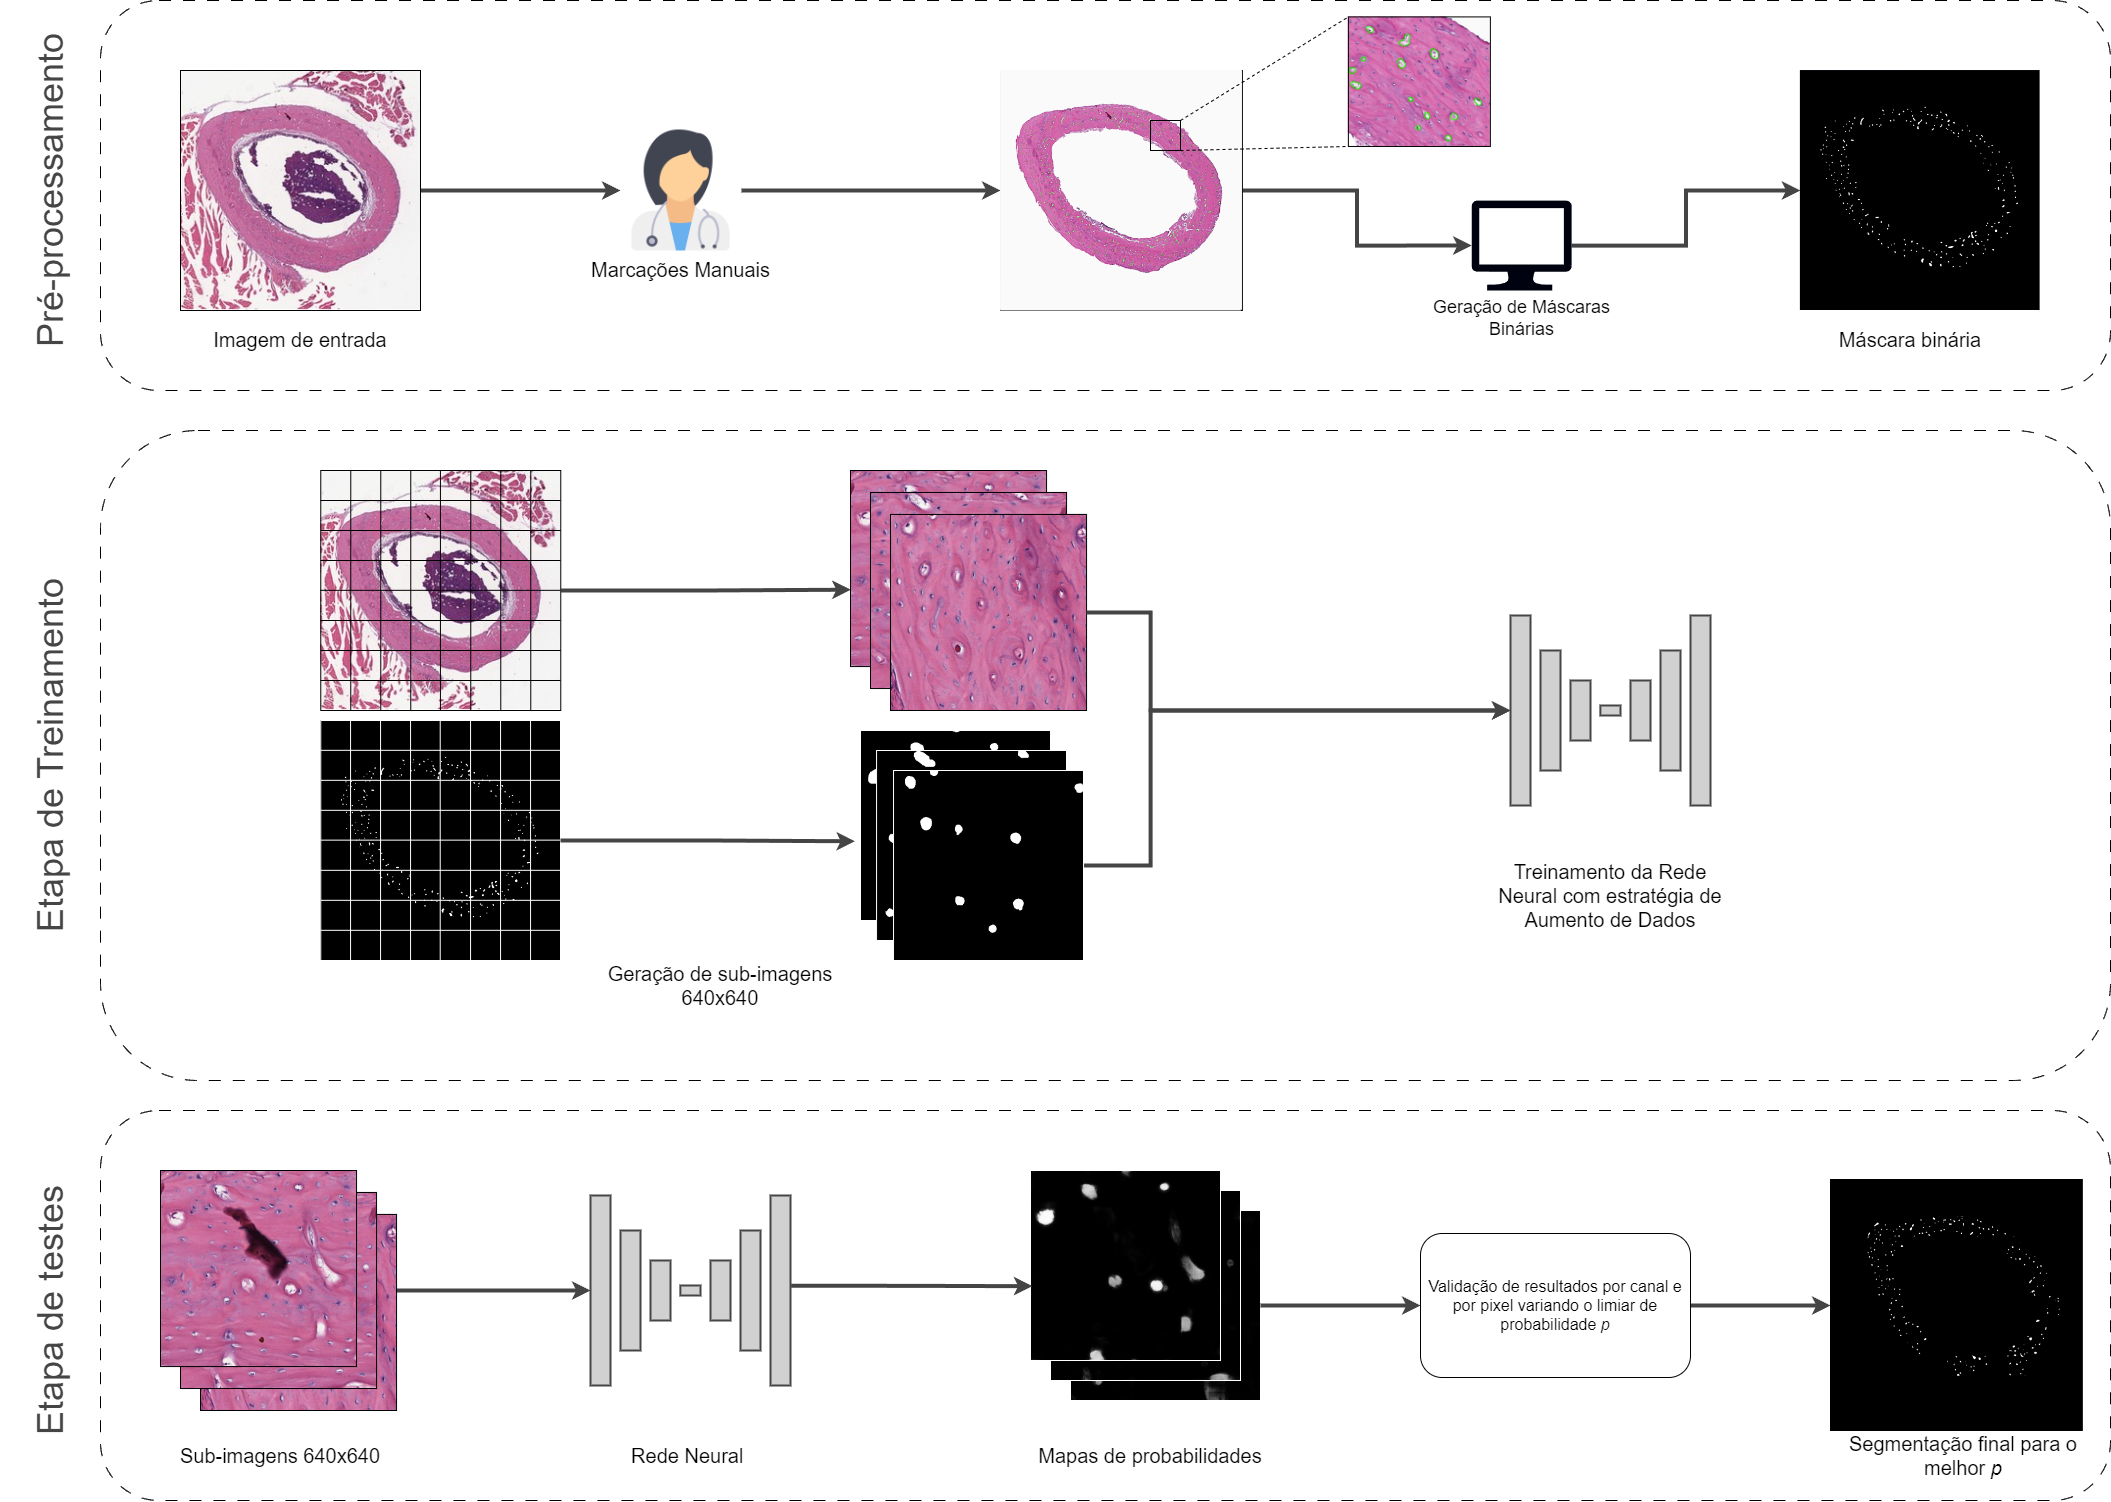
\includegraphics[width=1.25\textwidth]{figures/3_methods/metodologia.drawio.png}   
  
    \caption[Diagrama do método proposto.]{Metodologia utilizada. Inicialmente as imagens foram marcadas manualmente. Máscaras binárias foram geradas destacando as estruturas de interesse. A rede neural foi então treinada utilizando sub-imagens das imagens originais e suas máscaras; o treinamento contou com uma estratégia de aumento de dados. Mapas de probabilidades foram computados utilizando a rede treinada; diferentes valores de limiar de probabilidade $p$ foram testados em dois tipos de análise: pixel a pixel e canal a canal; a segmentação final foi feita utilizando o valor de $p$ que apresentou melhores resultados. }
    \label{fig:methodology-schema}
\end{figure}

\end{landscape}

%    \caption[Diagrama do método proposto.]{Diagrama da metodologia utilizada. Na etapa de preparo do conjunto de dados as imagens foram marcadas manualmente, e foram geradas máscaras binárias destacando as estruturas de interesse. Para a etapa de treinamento a rede neural foi treinada utilizando as sub-imagens das imagens originais e suas respectivas máscaras; o treinamento contou ainda com uma estratégia de aumento de dados. Na etapa de testes foram computados mapas de probabilidades utilizando a rede treinada; foram testados vários valores de limiar de probabilidade em dois tipos de análise: pixel a pixel e canal a canal; a segmentação final foi feita utilizando o limiar de probabilidade que apresentou melhores resultados. }


% ----------------------------------------------------------
% Experimentos e avaliação dos resultados
% ----------------------------------------------------------

\chapter[Resultados e Discussão]{Resultados e Discussão}
\label{resultados-e-discussao}

Este capítulo apresenta os resultados obtidos nos experimentos descritos no capítulo anterior.

\section{Treinamento da Rede}

Para a fase de treinamento, embora os resultados obtidos o \acs{TTA} tenham sido ligeiramente inferiores que os obtidos em \acs{TZ}, os rseultados foram semelhantes, e não houve mudança significativa na curva de aprendizado da rede. Para ambos os treinamentos foram obtidos sobre o conjunto de validação acurácia acima de 97\% e erro em torno de 12\%. A Figura~\ref{fig:640-acc-loss} mostra as curvas de perda e acurácia para ambos os conjuntos de dados ao longo de ambos os treinamentos.

\begin{figure}[h]
    \center
    \begin{tabular}{@{}c@{}}
        \includegraphics[width=0.9\textwidth]{figures/4_results/both_training_pt.png}
        \\[\abovecaptionskip]
    \end{tabular}
  
    \caption[Curvas de acurácia e perda ao logo do treinamento.]{Curvas de acurácia e perda ao logo de ambos os treinamentos. À esquerda a acurácia das previsões da rede aplicadas ao conjunto de treinamento (em azul para o \acs{TZ} e em laranja para o \acs{TTA}) e ao conjunto de validação (em verde para o \acs{TZ} e em vermelho para o \acs{TTA}). À direita a perda das previsões da rede aplicadas ao conjunto de treinamento (em azul para o \acs{TZ} e em laranja para o \acs{TTA}) e ao conjunto de validação (em verde para o \acs{TZ} e em vermelho para o \acs{TTA}).}
    \label{fig:640-acc-loss}
\end{figure}

A acurácia apresenta valores elevados principalmente devido ao desbalanceamento do conjunto de dados, pois as imagens possuem muito mais pixels negativos do que positivos, visto que os canais ósseos são estruturas pequenas que ocupam pouco espaço nas imagens quando comparamos à matriz óssea, por exemplo. 

\section{Análise por pixel}

Em seguida foi executada a inferência sobre as imagens do conjunto de testes. Nesta etapa a saída da rede neural é uma imagem em escala de cinza onde cada pixel possui um valor entre 0 e 255 e quanto maior a probabilidade de um pixel pertencer à região de interesse maior será o seu valor. Portanto, visualmente, quanto mais próximo da cor branca for o \textit{pixel} na imagem de saída maior a probabilidade de o mesmo pertencer à região de interesse, conforme ilustrado pela Figura \ref{fig:masks-result-and-original-640-202-r2c1}.

\begin{figure}[h]
    \center
    \begin{tabular}{@{}c@{}}
        \includegraphics[width=0.3\textwidth]{figures/4_results/network_640_mask.png}
        \\[\abovecaptionskip]
    \small (a)
    \end{tabular}
    \begin{tabular}{@{}c@{}}
        \includegraphics[width=0.3\textwidth]{figures/4_results/manual_640_mask.png}
        \\[\abovecaptionskip]
    \small (b)
    \end{tabular}
    \caption[Saída da rede neural.]{Saída da rede neural. Em (a) um exemplo de uma saída da rede neural. Em (b) a respectiva máscara manualmente marcada pelo especialista.}
    \label{fig:masks-result-and-original-640-202-r2c1}
\end{figure}

Dessa forma, um \textit{pixel} é considerado um positivo se a probabilidade de o mesmo pertencer à região de interesse for maior que um limiar $p$.

\begin{equation}
Y(x) = \left \{ \begin{matrix} 0, & \mbox{se } \frac{x}{255} < p
\\ 1, & \mbox{caso contrário} \end{matrix} \right. 
\label{eq-prob-threshold}
\end{equation}

Para validar o melhor valor para tal limiar foram testados vários valores de $p$, variando-o de 0,05 até 0,95 com um passo de 0,05. Para cada valor testado foram calculados os valores médios de acurácia, precisão, \textit{f1-score}, sensibilidade e especificidade. A Tabela \ref{tab:metricas-variando-p} e o gráfico da Figura \ref{fig:graphic-results} mostram os valores médios obtidos para cada valor de $p$.

% Please add the following required packages to your document preamble:
% \usepackage[table,xcdraw]{xcolor}
% If you use beamer only pass "xcolor=table" option, i.e. \documentclass[xcolor=table]{beamer}
\begin{table}

    \begin{small}
    \begin{tabular}{l|l|l|l|l|l|l|l|l|l|l}
    %\hline
    \rowcolor[HTML]{EFEFEF} \multicolumn{1}{c}{\cellcolor[HTML]{FFFFFF} } & \multicolumn{5}{c|}{\textbf{Treinamento do Zero}} & \multicolumn{5}{|c}{\textbf{Treinamento transferido}} \\ 
    \cline{1-11}
    \cline{1-11}
    \hline
    \textbf{\textit{p}}                     & \textbf{Acur.}                                & \textbf{Prec.}                              & \textbf{F1}                                       & \textbf{Sensib.}                                 & \textbf{Espec.}                               &\textbf{Acur.}                                 & \textbf{Prec.}                              & \textbf{F1}                                      & \textbf{Sensib.}                                 & \textbf{Espec.}     \\ \hline
    %\cellcolor[HTML]{EFEFEF}\textbf{0.00}  & \cellcolor[HTML]{FFEEEE}0.801                 & \cellcolor[HTML]{FFEEEE}0.154               & \cellcolor[HTML]{FFEEEE}0.257                     & \cellcolor[HTML]{FFEEEE}0.968                    & \cellcolor[HTML]{FFEEEE}0.796                 & \cellcolor[HTML]{EEFFEE}0.878                 & \cellcolor[HTML]{EEFFEE}0.217               & \cellcolor[HTML]{EEFFEE}0.340                    & \cellcolor[HTML]{EEFFEE}0.946                    & \cellcolor[HTML]{EEFFEE}0.881                       \\ \cline{1-11}
    \cellcolor[HTML]{EFEFEF}\textbf{0.05}   & \cellcolor[HTML]{FFEEEE}0.944                 & \cellcolor[HTML]{FFEEEE}0.416               & \cellcolor[HTML]{FFEEEE}0.548                     & \cellcolor[HTML]{FFEEEE}0.907                    & \cellcolor[HTML]{FFEEEE}0.953                 & \cellcolor[HTML]{EEFFEE}0.953                 & \cellcolor[HTML]{EEFFEE}0.450               & \cellcolor[HTML]{EEFFEE}0.580                    & \cellcolor[HTML]{EEFFEE}0.904                    & \cellcolor[HTML]{EEFFEE}0.962                       \\ \cline{1-11}
    \cellcolor[HTML]{EFEFEF}\textbf{0.10}   & \cellcolor[HTML]{FFEEEE}0.958                 & \cellcolor[HTML]{FFEEEE}0.505               & \cellcolor[HTML]{FFEEEE}0.615                     & \cellcolor[HTML]{FFEEEE}0.873                    & \cellcolor[HTML]{FFEEEE}0.969                 & \cellcolor[HTML]{EEFFEE}0.961                 & \cellcolor[HTML]{EEFFEE}0.520               & \cellcolor[HTML]{EEFFEE}0.632                    & \cellcolor[HTML]{EEFFEE}0.883                    & \cellcolor[HTML]{EEFFEE}0.972                       \\ \cline{1-11}
    \cellcolor[HTML]{EFEFEF}\textbf{0.15}   & \cellcolor[HTML]{FFEEEE}0.965                 & \cellcolor[HTML]{FFEEEE}0.563               & \cellcolor[HTML]{FFEEEE}0.651                     & \cellcolor[HTML]{FFEEEE}0.844                    & \cellcolor[HTML]{FFEEEE}0.977                 & \cellcolor[HTML]{EEFFEE}0.965                 & \cellcolor[HTML]{EEFFEE}0.564               & \cellcolor[HTML]{EEFFEE}0.660                    & \cellcolor[HTML]{EEFFEE}0.865                    & \cellcolor[HTML]{EEFFEE}0.977                       \\ \cline{1-11} 
    \cellcolor[HTML]{EFEFEF}\textbf{0.20}   & \cellcolor[HTML]{FFEEEE}0.968                 & \cellcolor[HTML]{FFEEEE}0.608               & \cellcolor[HTML]{FFEEEE}0.673                     & \cellcolor[HTML]{FFEEEE}0.817                    & \cellcolor[HTML]{FFEEEE}0.982                 & \cellcolor[HTML]{EEFFEE}0.968                 & \cellcolor[HTML]{EEFFEE}0.595               & \cellcolor[HTML]{EEFFEE}0.678                    & \cellcolor[HTML]{EEFFEE}0.850                    & \cellcolor[HTML]{EEFFEE}0.981                       \\ \cline{1-11}
    \cellcolor[HTML]{EFEFEF}\textbf{0.25}   & \cellcolor[HTML]{FFEEEE}0.970                 & \cellcolor[HTML]{FFEEEE}0.642               & \cellcolor[HTML]{FFEEEE}0.685                     & \cellcolor[HTML]{FFEEEE}0.794                    & \cellcolor[HTML]{FFEEEE}0.985                 & \cellcolor[HTML]{EEFFEE}0.970                 & \cellcolor[HTML]{EEFFEE}0.620               & \cellcolor[HTML]{EEFFEE}0.689                    & \cellcolor[HTML]{EEFFEE}0.836                    & \cellcolor[HTML]{EEFFEE}0.983                       \\ \cline{1-11}
    \cellcolor[HTML]{EFEFEF}\textbf{0.30}   & \cellcolor[HTML]{FFEEEE}0.971                 & \cellcolor[HTML]{FFEEEE}0.674               & \cellcolor[HTML]{FFEEEE}0.693                     & \cellcolor[HTML]{FFEEEE}0.769                    & \cellcolor[HTML]{FFEEEE}0.987                 & \cellcolor[HTML]{EEFFEE}0.971                 & \cellcolor[HTML]{EEFFEE}0.642               & \cellcolor[HTML]{EEFFEE}0.699                    & \cellcolor[HTML]{EEFFEE}0.822                    & \cellcolor[HTML]{EEFFEE}0.985                       \\ \cline{1-11}
    \cellcolor[HTML]{D8D8D8}\textbf{0.35}   & \cellcolor[HTML]{FFEEEE}0.972                 & \cellcolor[HTML]{FFEEEE}0.701               & \cellcolor[HTML]{FFDDDD}{\textbf{0.697}}          & \cellcolor[HTML]{FFEEEE}0.743                    & \cellcolor[HTML]{FFEEEE}0.989                 & \cellcolor[HTML]{EEFFEE}0.972                 & \cellcolor[HTML]{EEFFEE}0.663               & \cellcolor[HTML]{EEFFEE}0.705                    & \cellcolor[HTML]{EEFFEE}0.807                    & \cellcolor[HTML]{EEFFEE}0.987                       \\ \cline{1-11} 
    \cellcolor[HTML]{EFEFEF}\textbf{0.40}   & \cellcolor[HTML]{FFEEEE}0.973                 & \cellcolor[HTML]{FFEEEE}0.726               & \cellcolor[HTML]{FFEEEE}0.696                     & \cellcolor[HTML]{FFEEEE}0.716                    & \cellcolor[HTML]{FFEEEE}0.991                 & \cellcolor[HTML]{EEFFEE}0.973                 & \cellcolor[HTML]{EEFFEE}0.681               & \cellcolor[HTML]{EEFFEE}0.710                    & \cellcolor[HTML]{EEFFEE}0.792                    & \cellcolor[HTML]{EEFFEE}0.988                       \\ \cline{1-11}
    \cellcolor[HTML]{EFEFEF}\textbf{0.45}   & \cellcolor[HTML]{FFEEEE}0.973                 & \cellcolor[HTML]{FFEEEE}0.747               & \cellcolor[HTML]{FFEEEE}0.693                     & \cellcolor[HTML]{FFEEEE}0.689                    & \cellcolor[HTML]{FFEEEE}0.992                 & \cellcolor[HTML]{EEFFEE}0.973                 & \cellcolor[HTML]{EEFFEE}0.698               & \cellcolor[HTML]{EEFFEE}0.714                    & \cellcolor[HTML]{EEFFEE}0.779                    & \cellcolor[HTML]{EEFFEE}0.989                       \\ \cline{1-11}
    \cellcolor[HTML]{D8D8D8}\textbf{0.50}   & \cellcolor[HTML]{FFEEEE}0.973                 & \cellcolor[HTML]{FFEEEE}0.768               & \cellcolor[HTML]{FFEEEE}0.684                     & \cellcolor[HTML]{FFEEEE}0.657                    & \cellcolor[HTML]{FFEEEE}0.993                 & \cellcolor[HTML]{EEFFEE}0.974                 & \cellcolor[HTML]{EEFFEE}0.715               & \cellcolor[HTML]{DDFFDD}{\textbf{0.716}}         & \cellcolor[HTML]{EEFFEE}0.763                    & \cellcolor[HTML]{EEFFEE}0.990                       \\ \cline{1-11}
    \cellcolor[HTML]{EFEFEF}\textbf{0.55}   & \cellcolor[HTML]{FFEEEE}0.973                 & \cellcolor[HTML]{FFEEEE}0.789               & \cellcolor[HTML]{FFEEEE}0.671                     & \cellcolor[HTML]{FFEEEE}0.621                    & \cellcolor[HTML]{FFEEEE}0.995                 & \cellcolor[HTML]{EEFFEE}0.974                 & \cellcolor[HTML]{EEFFEE}0.731               & \cellcolor[HTML]{EEFFEE}0.715                    & \cellcolor[HTML]{EEFFEE}0.746                    & \cellcolor[HTML]{EEFFEE}0.991                       \\ \cline{1-11} 
    \cellcolor[HTML]{EFEFEF}\textbf{0.60}   & \cellcolor[HTML]{FFEEEE}0.973                 & \cellcolor[HTML]{FFEEEE}0.810               & \cellcolor[HTML]{FFEEEE}0.652                     & \cellcolor[HTML]{FFEEEE}0.580                    & \cellcolor[HTML]{FFEEEE}0.996                 & \cellcolor[HTML]{EEFFEE}0.975                 & \cellcolor[HTML]{EEFFEE}0.747               & \cellcolor[HTML]{EEFFEE}0.713                    & \cellcolor[HTML]{EEFFEE}0.725                    & \cellcolor[HTML]{EEFFEE}0.992                       \\ \cline{1-11}
    \cellcolor[HTML]{EFEFEF}\textbf{0.65}   & \cellcolor[HTML]{FFEEEE}0.972                 & \cellcolor[HTML]{FFEEEE}0.829               & \cellcolor[HTML]{FFEEEE}0.628                     & \cellcolor[HTML]{FFEEEE}0.537                    & \cellcolor[HTML]{FFEEEE}0.996                 & \cellcolor[HTML]{EEFFEE}0.975                 & \cellcolor[HTML]{EEFFEE}0.763               & \cellcolor[HTML]{EEFFEE}0.709                    & \cellcolor[HTML]{EEFFEE}0.705                    & \cellcolor[HTML]{EEFFEE}0.993                       \\ \cline{1-11}
    \cellcolor[HTML]{EFEFEF}\textbf{0.70}   & \cellcolor[HTML]{FFEEEE}0.971                 & \cellcolor[HTML]{FFEEEE}0.840               & \cellcolor[HTML]{FFEEEE}0.592                     & \cellcolor[HTML]{FFEEEE}0.484                    & \cellcolor[HTML]{FFEEEE}0.997                 & \cellcolor[HTML]{EEFFEE}0.975                 & \cellcolor[HTML]{EEFFEE}0.779               & \cellcolor[HTML]{EEFFEE}0.702                    & \cellcolor[HTML]{EEFFEE}0.679                    & \cellcolor[HTML]{EEFFEE}0.994                       \\ \cline{1-11}
    \cellcolor[HTML]{EFEFEF}\textbf{0.75}   & \cellcolor[HTML]{FFEEEE}0.970                 & \cellcolor[HTML]{FFEEEE}0.858               & \cellcolor[HTML]{FFEEEE}0.547                     & \cellcolor[HTML]{FFEEEE}0.426                    & \cellcolor[HTML]{FFEEEE}0.998                 & \cellcolor[HTML]{EEFFEE}0.975                 & \cellcolor[HTML]{EEFFEE}0.796               & \cellcolor[HTML]{EEFFEE}0.692                    & \cellcolor[HTML]{EEFFEE}0.650                    & \cellcolor[HTML]{EEFFEE}0.995                       \\ \cline{1-11} 
    \cellcolor[HTML]{EFEFEF}\textbf{0.80}   & \cellcolor[HTML]{FFEEEE}0.969                 & \cellcolor[HTML]{FFEEEE}0.873               & \cellcolor[HTML]{FFEEEE}0.487                     & \cellcolor[HTML]{FFEEEE}0.360                    & \cellcolor[HTML]{FFEEEE}0.998                 & \cellcolor[HTML]{EEFFEE}0.974                 & \cellcolor[HTML]{EEFFEE}0.814               & \cellcolor[HTML]{EEFFEE}0.677                    & \cellcolor[HTML]{EEFFEE}0.616                    & \cellcolor[HTML]{EEFFEE}0.996                       \\ \cline{1-11}
    \cellcolor[HTML]{EFEFEF}\textbf{0.85}   & \cellcolor[HTML]{FFEEEE}0.967                 & \cellcolor[HTML]{FFEEEE}0.882               & \cellcolor[HTML]{FFEEEE}0.415                     & \cellcolor[HTML]{FFEEEE}0.290                    & \cellcolor[HTML]{FFEEEE}0.999                 & \cellcolor[HTML]{EEFFEE}0.974                 & \cellcolor[HTML]{EEFFEE}0.834               & \cellcolor[HTML]{EEFFEE}0.653                    & \cellcolor[HTML]{EEFFEE}0.571                    & \cellcolor[HTML]{EEFFEE}0.997                       \\ \cline{1-11}
    \cellcolor[HTML]{EFEFEF}\textbf{0.90}   & \cellcolor[HTML]{FFEEEE}0.965                 & \cellcolor[HTML]{FFEEEE}0.884               & \cellcolor[HTML]{FFEEEE}0.303                     & \cellcolor[HTML]{FFEEEE}0.195                    & \cellcolor[HTML]{FFEEEE}0.999                 & \cellcolor[HTML]{EEFFEE}0.973                 & \cellcolor[HTML]{EEFFEE}0.851               & \cellcolor[HTML]{EEFFEE}0.613                    & \cellcolor[HTML]{EEFFEE}0.507                    & \cellcolor[HTML]{EEFFEE}0.998                       \\ \cline{1-11}
    \cellcolor[HTML]{EFEFEF}\textbf{0.95}   & \cellcolor[HTML]{FFEEEE}0.962                 & \cellcolor[HTML]{FFEEEE}0.780               & \cellcolor[HTML]{FFEEEE}0.135                     & \cellcolor[HTML]{FFEEEE}0.078                    & \cellcolor[HTML]{FFEEEE}0.999                 & \cellcolor[HTML]{EEFFEE}0.970                 & \cellcolor[HTML]{EEFFEE}0.880               & \cellcolor[HTML]{EEFFEE}0.509                    & \cellcolor[HTML]{EEFFEE}0.378                    & \cellcolor[HTML]{EEFFEE}0.999                       \\ \cline{1-11}
    \end{tabular}
    \end{small}
    \caption{Médias de acurácia, precisão, \textit{f1-score}, sensibilidade e especificidade para cada \textit{threshold} $p$ testado na análise por pixel.}
        \label{tab:metricas-variando-p}
\end{table}

\begin{figure}
    \center
    \includegraphics[width=0.9\textwidth]{figures/4_results/TTZ - Medidas x p (análise por pixel).png}
  
    \includegraphics[width=0.9\textwidth]{figures/4_results/TTA - Medidas x p (análise por pixel).png}
  
    \caption[Métricas obtidas na análise por pixel de ambos os treinamentos.]{Acurácia, \textit{f1-score}, precisão, sensibilidade e especificidade em função do \textit{threshold} $p$ na análise por pixel de ambos os treinamentos.}
    \label{fig:graphic-results}
\end{figure}

Após o teste foi observado que o \acs{TTA} obteve resultados melhores que o \acs{TZ}, alcançando 71,6\% para $p$=0,5 de \textit{f1-score}, logo, a melhor relação entre precisão e sensibilidade. A especificidade e acurácia se mantiveram elevadas durante todo o teste devido ao alto volume de \textit{pixels} negativos corretamente classificados.

Utilizando o resultado acima foi feita a segmentação das imagens do conjunto de testes utilizando o modelo treinado a partir do zero com $p$=0,35. A Figura \ref{fig:marcacoes-final} compara a máscara gerada pela rede com a máscara gerada a partir das marcações do especialista, e a Figura \ref{fig:marcacoes-final-regioes} mostra uma imagem da lâmina inteira marcada a partir da máscara gerada pela rede e algumas regiões ampliadas para detalhar os resultados, em que ainda é possível observar alguns falsos negativos.

\begin{figure}
    \center
    \begin{tabular}{@{}c@{}}
        \includegraphics[width=0.9\textwidth]{figures/4_results/figure-manuel-net-results-comparision_lower_res.png}
        \\[\abovecaptionskip]
    \end{tabular}
  
    \caption[Comparação entre marcação manual feita por especialista e saída do método.]{Comparação entre marcação manual feita por especialista e saída do método. Na primeira coluna exemplos de marcações manuais, na segunda coluna as máscaras geradas pelo método treinado a partir do zero e com um limiar $p$=0,35. Imagem em resolução original disponível \href{https://github.com/igorgonribs/dissertacao/blob/master/figures/4_results/figure-manuel-net-results-comparision.png}{neste link}}
    \label{fig:marcacoes-final}
\end{figure}


\begin{figure}
    \center
    \includegraphics[width=0.8\textwidth]{figures/4_results/302areas_reduzida.png}
   
    \caption[Imagem marcada pela rede com regiões ampliadas]{Imagem de lâmina inteira com as marcações feitas pela rede em verde e com três regiões ampliadas. Observa-se, principalmente na região delimitada pela cor azul, a presença de alguns falsos negativos.}
    \label{fig:marcacoes-final-regioes}
\end{figure}


\section{Análise por canal}

Nesta análise, para cada componente conectado da máscara de referência foi extraída uma sub-imagem de acordo com as coordenadas \(x_i, x_f, y_i, y_f\) do componente, em que $x_i$  e $y_i$ representam o menor valor de coordenada do pixel em x e y,  enquanto $x_f$ e $y_f$ representam o maior valor de coordenada do pixel em x e y. Extraía-se também uma sub-imagem da respectiva região delimitada por \(x_i, x_f, y_i, y_f\) na imagem segmentada pelo método para verificar se havia ou não um canal naquela região. Em seguida foi calculada a intersecção entre entre as duas sub-imagens. Foram considerados como verdadeiros positivos os componentes cuja intersecção coincidiram ao menos 70\% com o canal da máscara de referência. A Figura \ref{fig:intersection-net} mostra exemplos de canais na máscara de referência, na segmentação da rede e a intersecção entre os dois canais. 

\begin{figure}
    \centering
    
    \begin{tabular}{@{}c@{}}
        \includegraphics[width=0.5\textwidth]{figures/4_results/components/305_r10c7_component_1.png} \\
        \includegraphics[width=0.5\textwidth]{figures/4_results/components/305_r11c7_component_1.png} \\
        \includegraphics[width=0.5\textwidth]{figures/4_results/components/305_r12c11_component_1.png} 
    \end{tabular}

    \caption[Exemplos de componentes conectados obtidos pelo método proposto.]{Três exemplos de componentes conectados analisados durante a análise por canal. Na primeira coluna o componente na máscara de referência em amarelo (padrão ouro). Na segunda coluna a segmentação da rede neural para o respectivo componente. Na terceira coluna a intersecção entre a primeira e a segunda coluna.}
    \label{fig:intersection-net}
\end{figure}

Em seguida foram extraídas da imagem segmentada sub-imagens representando os componentes conectados que não estavam presentes na imagem de referência, identificando, portanto, os falsos positivos. Nessa análise não é possível contabilizar verdadeiros negativos. 


Para essa nova análise foram testados novamente os valores do limiar de probabilidade $p$. Por não termos o número de verdadeiros negativos as métricas utilizadas foram: Precisão, \textit{f1-score}, sensibilidade e Intersecção sobre União. O melhor resultado para ambos os treinamentos foi obtido para \(p = 0,10\). A Tabela \ref{tab:metricas-variando-p-por-canal} mostra o resultados da análise para cada valor de $p$ em ambos os treinamentos.

\begin{table}[h]
    \center
    \begin{small}
    \begin{tabular}{|l|l|l|l|l|l|l|l|l|l|}
        \multicolumn{1}{c}{\cellcolor[HTML]{FFFFFF} } & \multicolumn{4}{c|}{\cellcolor[HTML]{FFEEEE}\textbf{Treinamento do Zero}} & \multicolumn{4}{|c}{\cellcolor[HTML]{EEFFEE}\textbf{Treinamento transferido}} \\ 
        \cline{1-9}
        \cline{1-9}
\hline

\cellcolor[HTML]{D8D8D8}\textbf{\textit{p}}    &  \cellcolor[HTML]{FFDDDD}\textbf{Precisão}   & \cellcolor[HTML]{FFDDDD}\textbf{F1-Score}  & \cellcolor[HTML]{FFDDDD}\textbf{Sensibilidade}    & \cellcolor[HTML]{FFDDDD}\textbf{IoU}       &  \cellcolor[HTML]{DDFFDD}\textbf{Precisão}   & \cellcolor[HTML]{DDFFDD}\textbf{F1-Score}  & \cellcolor[HTML]{DDFFDD}\textbf{Sensibilidade}   & \cellcolor[HTML]{DDFFDD}\textbf{IoU}       \\ \hline
%\cellcolor[HTML]{EFEFEF}\textbf{0.00}   &  \cellcolor[HTML]{FFEEEE}0.772               & \cellcolor[HTML]{FFEEEE}0.837              & \cellcolor[HTML]{FFEEEE}0.965                     & \cellcolor[HTML]{FFEEEE}0.718              &  \cellcolor[HTML]{EEFFEE}0.728               & \cellcolor[HTML]{EEFFEE}0.805              & \cellcolor[HTML]{EEFFEE}0.958                    & \cellcolor[HTML]{EEFFEE}0.677              \\ \cline{1-9}
\cellcolor[HTML]{EFEFEF}\textbf{0.05}   &  \cellcolor[HTML]{FFEEEE}0.805               & \cellcolor[HTML]{FFEEEE}0.831              & \cellcolor[HTML]{FFEEEE}0.896                     & \cellcolor[HTML]{FFEEEE}0.718              &  \cellcolor[HTML]{EEFFEE}0.833               & \cellcolor[HTML]{EEFFEE}0.860              & \cellcolor[HTML]{EEFFEE}0.917                    & \cellcolor[HTML]{EEFFEE}0.774              \\ \cline{1-9}
\cellcolor[HTML]{D8D8D8}\textbf{0.10}   &  \cellcolor[HTML]{FFEEEE}0.836               & \cellcolor[HTML]{FFDDDD}{\textbf{0.838}}   & \cellcolor[HTML]{FFEEEE}0.866                     & \cellcolor[HTML]{FFDDDD}{\textbf{0.737}}   &  \cellcolor[HTML]{EEFFEE}0.856               & \cellcolor[HTML]{DDFFDD}{\textbf{0.863}}   & \cellcolor[HTML]{EEFFEE}0.898                    & \cellcolor[HTML]{DDFFDD}{\textbf{0.782}}   \\ \cline{1-9}
\cellcolor[HTML]{EFEFEF}\textbf{0.15}   &  \cellcolor[HTML]{FFEEEE}0.844               & \cellcolor[HTML]{FFEEEE}0.826              & \cellcolor[HTML]{FFEEEE}0.835                     & \cellcolor[HTML]{FFEEEE}0.720              &  \cellcolor[HTML]{EEFFEE}0.867               & \cellcolor[HTML]{EEFFEE}0.863              & \cellcolor[HTML]{EEFFEE}0.883                    & \cellcolor[HTML]{EEFFEE}0.781              \\ \cline{1-9} 
\cellcolor[HTML]{EFEFEF}\textbf{0.20}   &  \cellcolor[HTML]{FFEEEE}0.846               & \cellcolor[HTML]{FFEEEE}0.812              & \cellcolor[HTML]{FFEEEE}0.806                     & \cellcolor[HTML]{FFEEEE}0.702              &  \cellcolor[HTML]{EEFFEE}0.871               & \cellcolor[HTML]{EEFFEE}0.857              & \cellcolor[HTML]{EEFFEE}0.867                    & \cellcolor[HTML]{EEFFEE}0.775              \\ \cline{1-9}
\cellcolor[HTML]{EFEFEF}\textbf{0.25}   &  \cellcolor[HTML]{FFEEEE}0.844               & \cellcolor[HTML]{FFEEEE}0.796              & \cellcolor[HTML]{FFEEEE}0.778                     & \cellcolor[HTML]{FFEEEE}0.679              &  \cellcolor[HTML]{EEFFEE}0.873               & \cellcolor[HTML]{EEFFEE}0.850              & \cellcolor[HTML]{EEFFEE}0.850                    & \cellcolor[HTML]{EEFFEE}0.765              \\ \cline{1-9}
\cellcolor[HTML]{EFEFEF}\textbf{0.30}   &  \cellcolor[HTML]{FFEEEE}0.846               & \cellcolor[HTML]{FFEEEE}0.780              & \cellcolor[HTML]{FFEEEE}0.748                     & \cellcolor[HTML]{FFEEEE}0.660              &  \cellcolor[HTML]{EEFFEE}0.877               & \cellcolor[HTML]{EEFFEE}0.843              & \cellcolor[HTML]{EEFFEE}0.835                    & \cellcolor[HTML]{EEFFEE}0.756              \\ \cline{1-9}
\cellcolor[HTML]{EFEFEF}\textbf{0.35}   &  \cellcolor[HTML]{FFEEEE}0.837               & \cellcolor[HTML]{FFEEEE}0.756              & \cellcolor[HTML]{FFEEEE}0.713                     & \cellcolor[HTML]{FFEEEE}0.631              &  \cellcolor[HTML]{EEFFEE}0.873               & \cellcolor[HTML]{EEFFEE}0.831              & \cellcolor[HTML]{EEFFEE}0.815                    & \cellcolor[HTML]{EEFFEE}0.738              \\ \cline{1-9} 
\cellcolor[HTML]{EFEFEF}\textbf{0.40}   &  \cellcolor[HTML]{FFEEEE}0.827               & \cellcolor[HTML]{FFEEEE}0.730              & \cellcolor[HTML]{FFEEEE}0.678                     & \cellcolor[HTML]{FFEEEE}0.595              &  \cellcolor[HTML]{EEFFEE}0.871               & \cellcolor[HTML]{EEFFEE}0.819              & \cellcolor[HTML]{EEFFEE}0.797                    & \cellcolor[HTML]{EEFFEE}0.725              \\ \cline{1-9}
\cellcolor[HTML]{EFEFEF}\textbf{0.45}   &  \cellcolor[HTML]{FFEEEE}0.813               & \cellcolor[HTML]{FFEEEE}0.698              & \cellcolor[HTML]{FFEEEE}0.637                     & \cellcolor[HTML]{FFEEEE}0.555              &  \cellcolor[HTML]{EEFFEE}0.871               & \cellcolor[HTML]{EEFFEE}0.811              & \cellcolor[HTML]{EEFFEE}0.783                    & \cellcolor[HTML]{EEFFEE}0.713              \\ \cline{1-9}
\cellcolor[HTML]{EFEFEF}\textbf{0.50}   &  \cellcolor[HTML]{FFEEEE}0.792               & \cellcolor[HTML]{FFEEEE}0.659              & \cellcolor[HTML]{FFEEEE}0.591                     & \cellcolor[HTML]{FFEEEE}0.508              &  \cellcolor[HTML]{EEFFEE}0.864               & \cellcolor[HTML]{EEFFEE}0.799              & \cellcolor[HTML]{EEFFEE}0.766                    & \cellcolor[HTML]{EEFFEE}0.695              \\ \cline{1-9}
\cellcolor[HTML]{EFEFEF}\textbf{0.55}   &  \cellcolor[HTML]{FFEEEE}0.770               & \cellcolor[HTML]{FFEEEE}0.614              & \cellcolor[HTML]{FFEEEE}0.538                     & \cellcolor[HTML]{FFEEEE}0.452              &  \cellcolor[HTML]{EEFFEE}0.854               & \cellcolor[HTML]{EEFFEE}0.783              & \cellcolor[HTML]{EEFFEE}0.745                    & \cellcolor[HTML]{EEFFEE}0.673              \\ \cline{1-9} 
\cellcolor[HTML]{EFEFEF}\textbf{0.60}   &  \cellcolor[HTML]{FFEEEE}0.748               & \cellcolor[HTML]{FFEEEE}0.563              & \cellcolor[HTML]{FFEEEE}0.477                     & \cellcolor[HTML]{FFEEEE}0.396              &  \cellcolor[HTML]{EEFFEE}0.847               & \cellcolor[HTML]{EEFFEE}0.765              & \cellcolor[HTML]{EEFFEE}0.720                    & \cellcolor[HTML]{EEFFEE}0.648              \\ \cline{1-9}
\cellcolor[HTML]{EFEFEF}\textbf{0.65}   &  \cellcolor[HTML]{FFEEEE}0.712               & \cellcolor[HTML]{FFEEEE}0.503              & \cellcolor[HTML]{FFEEEE}0.415                     & \cellcolor[HTML]{FFEEEE}0.340              &  \cellcolor[HTML]{EEFFEE}0.841               & \cellcolor[HTML]{EEFFEE}0.745              & \cellcolor[HTML]{EEFFEE}0.692                    & \cellcolor[HTML]{EEFFEE}0.625              \\ \cline{1-9}
\cellcolor[HTML]{EFEFEF}\textbf{0.70}   &  \cellcolor[HTML]{FFEEEE}0.660               & \cellcolor[HTML]{FFEEEE}0.434              & \cellcolor[HTML]{FFEEEE}0.347                     & \cellcolor[HTML]{FFEEEE}0.277              &  \cellcolor[HTML]{EEFFEE}0.823               & \cellcolor[HTML]{EEFFEE}0.712              & \cellcolor[HTML]{EEFFEE}0.654                    & \cellcolor[HTML]{EEFFEE}0.582              \\ \cline{1-9}
\cellcolor[HTML]{EFEFEF}\textbf{0.75}   &  \cellcolor[HTML]{FFEEEE}0.609               & \cellcolor[HTML]{FFEEEE}0.368              & \cellcolor[HTML]{FFEEEE}0.284                     & \cellcolor[HTML]{FFEEEE}0.218              &  \cellcolor[HTML]{EEFFEE}0.809               & \cellcolor[HTML]{EEFFEE}0.679              & \cellcolor[HTML]{EEFFEE}0.611                    & \cellcolor[HTML]{EEFFEE}0.540              \\ \cline{1-9} 
\cellcolor[HTML]{EFEFEF}\textbf{0.80}   &  \cellcolor[HTML]{FFEEEE}0.535               & \cellcolor[HTML]{FFEEEE}0.291              & \cellcolor[HTML]{FFEEEE}0.217                     & \cellcolor[HTML]{FFEEEE}0.163              &  \cellcolor[HTML]{EEFFEE}0.786               & \cellcolor[HTML]{EEFFEE}0.632              & \cellcolor[HTML]{EEFFEE}0.552                    & \cellcolor[HTML]{EEFFEE}0.482              \\ \cline{1-9}
\cellcolor[HTML]{EFEFEF}\textbf{0.85}   &  \cellcolor[HTML]{FFEEEE}0.420               & \cellcolor[HTML]{FFEEEE}0.200              & \cellcolor[HTML]{FFEEEE}0.142                     & \cellcolor[HTML]{FFEEEE}0.104              &  \cellcolor[HTML]{EEFFEE}0.743               & \cellcolor[HTML]{EEFFEE}0.570              & \cellcolor[HTML]{EEFFEE}0.487                    & \cellcolor[HTML]{EEFFEE}0.417              \\ \cline{1-9}
\cellcolor[HTML]{EFEFEF}\textbf{0.90}   &  \cellcolor[HTML]{FFEEEE}0.246               & \cellcolor[HTML]{FFEEEE}0.099              & \cellcolor[HTML]{FFEEEE}0.067                     & \cellcolor[HTML]{FFEEEE}0.046              &  \cellcolor[HTML]{EEFFEE}0.651               & \cellcolor[HTML]{EEFFEE}0.455              & \cellcolor[HTML]{EEFFEE}0.372                    & \cellcolor[HTML]{EEFFEE}0.298              \\ \cline{1-9}
\cellcolor[HTML]{EFEFEF}\textbf{0.95}   &  \cellcolor[HTML]{FFEEEE}0.055               & \cellcolor[HTML]{FFEEEE}0.017              & \cellcolor[HTML]{FFEEEE}0.011                     & \cellcolor[HTML]{FFEEEE}0.008              &  \cellcolor[HTML]{EEFFEE}0.362               & \cellcolor[HTML]{EEFFEE}0.209              & \cellcolor[HTML]{EEFFEE}0.158                    & \cellcolor[HTML]{EEFFEE}0.108              \\ \cline{1-9}
\end{tabular}
\end{small}
\caption{Médias de acurácia, precisão, \textit{f1-score}, sensibilidade e especificidade para cada \textit{threshold} $p$ testado na análise por canal.}
    \label{tab:metricas-variando-p-por-canal}
\end{table}

A análise descrita acima foi realizada sobre as imagens do conjunto de testes segmentadas com o limiar \(p = 0,10\). Novamente foi observado que o modelo \acs{TTA} apresentou resultados superiores ao modelo \acs{TZ}, obtendo 86,3\% e 78,2\% de \textit{f1-score} e Intersecção sobre União, respectivamente. Além disso na análise por canal houve um ganho significativo na \textit{f1-score} em relação ao melhor valor obtido na análise por pixel. A Figura \ref{fig:graphic-metrics-x-p-per-canal} mostra um gráfico com as medidas calculadas para cada valor de $p$ testado.

\begin{figure}
    \center
    \includegraphics[width=0.9\textwidth]{figures/4_results/TTZ - Medidas x p (análise por canal).png}

    \includegraphics[width=0.9\textwidth]{figures/4_results/TTA - Medidas x p (análise por canal).png}
  
    \caption[Métricas obtidas na análise por canal para ambos os treinamentos.]{Precisão, \textit{f1-score}, Intersecção sobre União e sensibilidade em função do \textit{threshold} $p$ na análise por canal de ambos os treinamentos.}
    \label{fig:graphic-metrics-x-p-per-canal}
\end{figure}


%Verdadeiros positivos: 3087
%Falsos negativos: 451
%Falsos positivos: 649
%Acurácia: 0.7372820635299737
%Sensibilidade: 0.8725268513284341
%Precisão: 0.8262847965738758
%F1-Score: 0.8487764641187792


A Figura \ref{fig:marcacoes-final-canal} mostra a comparação entre máscaras geradas a partir da marcação manual do especialista e máscaras geradas pelo método com $p$=0,1. Já a Figura \ref{fig:marcacoes-final-canal-regioes} mostra algumas regiões ampliadas para melhor visualização dos detalhes das marcações.

Na Figura~\ref{fig:marcacoes-final-canal} é possível encontrar algumas regiões escuras na matriz óssea indicando que não foram marcados canais nestas regiões. Este é possivelmente um ponto a melhorar no método, e uma das possíveis causas para essas lacunas é o tamanho das manchas. Talvez utilizando sub-imagens com tamanho 640x640 não tenha sido possível atingir granularidade suficiente para cobrir toda a matriz óssea.

\begin{figure}[h]
    \center
    \begin{tabular}{@{}c@{}}
        \includegraphics[width=0.25\textwidth]{figures/4_results/204_mask_manual_lower_res.png}
        \\[\abovecaptionskip]
    \end{tabular}
    \begin{tabular}{@{}c@{}}
        \includegraphics[width=0.25\textwidth]{figures/4_results/204_net_mask_gaps_lower_res.png}
        \\[\abovecaptionskip]
    \end{tabular}
    \begin{tabular}{@{}c@{}}
        \includegraphics[width=0.25\textwidth]{figures/4_results/204_marcacao_rede_inteira_10.png}
        \\[\abovecaptionskip]
    \end{tabular}

    \begin{tabular}{@{}c@{}}
        \includegraphics[width=0.25\textwidth]{figures/4_results/302_mask_manual_lower_res.png}
        \\[\abovecaptionskip]
    \end{tabular}
    \begin{tabular}{@{}c@{}}
        \includegraphics[width=0.25\textwidth]{figures/4_results/302_net_mask_gaps_lower_res.png}
        \\[\abovecaptionskip]
    \end{tabular}
    \begin{tabular}{@{}c@{}}
        \includegraphics[width=0.25\textwidth]{figures/4_results/302_marcacao_rede_inteira_10.png}
        \\[\abovecaptionskip]
    \end{tabular}
  
    \caption[Comparação entre marcação manual feita por especialista e saída do método.]{Comparação entre marcação manual feita por especialista e saída do método. Na primeira coluna exemplos de marcações manuais; na segunda coluna as máscaras geradas pelo método utilizando um limiar $p$=0,1 com algumas lacunas destacadas em vermelho; na terceira coluna a imagem marcada a partir da máscara gerada pela rede.}
    \label{fig:marcacoes-final-canal}
\end{figure}

\begin{figure}[h]
    \center
    \begin{tabular}{@{}c@{}}
        \includegraphics[width=0.25\textwidth]{figures/4_results/204_r3c2_mask_manual_10.png}
        \\[\abovecaptionskip]
    \end{tabular}
    \begin{tabular}{@{}c@{}}
        \includegraphics[width=0.25\textwidth]{figures/4_results/204_r3c2_mask_net_10.png}
        \\[\abovecaptionskip]
    \end{tabular}
    \begin{tabular}{@{}c@{}}
        \includegraphics[width=0.25\textwidth]{figures/4_results/204_r3c2_net_out_10.png}
        \\[\abovecaptionskip]
    \end{tabular}

    \begin{tabular}{@{}c@{}}
        \includegraphics[width=0.25\textwidth]{figures/4_results/204_r4c2_mask_manual_10.png}
        \\[\abovecaptionskip]
    \end{tabular}
    \begin{tabular}{@{}c@{}}
        \includegraphics[width=0.25\textwidth]{figures/4_results/204_r4c2_mask_net_10.png}
        \\[\abovecaptionskip]
    \end{tabular}
    \begin{tabular}{@{}c@{}}
        \includegraphics[width=0.25\textwidth]{figures/4_results/204_r4c2_net_out_10.png}
        \\[\abovecaptionskip]
    \end{tabular}
  
    \caption[Comparação de regiões ampliadas das marcações manuais feita por especialista e de saídas do método]{Comparação de regiões ampliadas das marcações manuais feita por especialista e de saídas do método. Na primeira coluna regiões ampliadas de marcações manuais, na segunda coluna as respectivas regiões nas máscaras geradas pelo método utilizando um limiar $p$=0,1, e na terceira coluna as respectivas regiões na imagens marcadas a partir das máscaras geradas pela rede.}
    \label{fig:marcacoes-final-canal-regioes}
\end{figure}

\subsection{Comparação}

A fim de comparação, foi feita uma implementação do algoritmo proposto por \cite{gondim2021automatic} utilizando a linguagem de programação Python na versão 3.10. As imagens de lâmina inteira do conjunto de testes foram então segmentadas e foi realizada a análise por canal conforme descrito anteriormente. A Figura \ref{fig:intersection-gondim} mostra exemplos de componentes conectados obtidos na análise por canal do algoritmo.


\begin{figure}[h]
    \centering
    
    \begin{tabular}{@{}c@{}}
        \includegraphics[width=0.6\textwidth]{figures/4_results/components/gondim_203_component_1.png} \\
        \includegraphics[width=0.6\textwidth]{figures/4_results/components/gondim_204_component_1.png} \\
        \includegraphics[width=0.6\textwidth]{figures/4_results/components/gondim_301_component_1.png} 
    \end{tabular}

    \caption[Exemplos de componentes conectados obtidos pelo método proposto por \cite{gondim2021automatic}.]{Três exemplos de componentes conectados analisados. Na primeira coluna o componente na máscara de referência (padrão ouro). Na segunda coluna a segmentação do algoritmo de \cite{gondim2021automatic} para o respectivo componente. Na terceira coluna a intersecção entre a primeira e a segunda coluna.}
    \label{fig:intersection-gondim}
\end{figure}

Foi observado que no método proposto neste trabalho era menos comum a aparição de falsos negativos. Além disso, algumas imagens do conjunto de testes apresentavam concavidades no formato do corte histológico e o método de \cite{gondim2021automatic} não reagiu bem para tais imagens, conforme mostrado na Figura \ref{fig:gondim-bad-prediction}.

\begin{figure}[h]
    \centering
    
    \begin{tabular}{c}
        \includegraphics[width=0.8\textwidth]{figures/4_results/falha-gondim_lower_res.png} \\[\abovecaptionskip]
    \small (a) 
    \end{tabular}

    \caption[Exemplo de falha do algoritmo proposto por \cite{gondim2021automatic}.]{Exemplo de falha do algoritmo proposto por \cite{gondim2021automatic}. Apesar de funcionar para cortes histológicos de formato convexo (sub-figuras (a) e (b)) o método falha ao trabalhar com cortes que apresentem concavidades (sub-figuras (c) e (d)).}
    \label{fig:gondim-bad-prediction}
\end{figure}

Os resultados obtidos em \cite{gondim2021automatic} mostram acurácia e especificidade próximas a 96\%, sensibilidade acima de 80\% e cerca de 90\% de \textit{f1-score}. Porém as marcações dos especialistas não seguiram a forma exata das estruturas, assim, foram considerados como verdadeiros positivos os canais cuja marcação do especialista estivesse ao menos 20\% contida na marcação feita pelo método. 

Não fica claro se as imagens utilizadas em \cite{gondim2021automatic} continham imagens de diferentes regiões da diáfise femoral -- região intermediária do fêmur. Devido à anatomia do osso, imagens provenientes da região central da diáfise resultam em cortes histológicos mais arredondados, semelhantes à Figura \ref{fig:gondim-bad-prediction}(a), enquanto imagens extraídas de regiões mais próximas às extremidades da diáfise podem resultar em cortes histológicos que apresentem outros formatos, como o observado na Figura \ref{fig:gondim-bad-prediction}(c). 

A análise por canal -- descrita na seção 4.2 -- da reprodução do algoritmo proposto por \cite{gondim2021automatic} apresentou um \textit{f1-score} de aproximadamente 17,5\% e uma Intersecção sobre União de 9,6\%. A Tabela \ref{tab:metricas-comparacao-por-canal} mostra os resultados obtidos pela análise por canal para cada um dos métodos. Vale ressaltar que esse valor é bem inferior ao obtido pelos autores pois neste trabalho são consideradas como válidas as intersecções que coincidem 70\% ou mais com o canal da máscara de referência, enquanto que no trabalho original era consideradas interseções de apenas 20\%.

%Verdadeiros positivos: 391
%Verdadeiros negativos: 3447
%Falsos positivos: 241
%Acurácia: 0.09585682765383673
%Sensibilidade: 0.10187597707139134
%Precisão: 0.6186708860759493
%F1-Score: 0.1749440715883669
%Jaccard: 0.095

% TABELA AQUI
\begin{table}[h]
\center
\begin{tiny}
\begin{tabular}{|l|l|l|l|l|}
\hline
\rowcolor[HTML]{C0C0C0} 
\textbf{Método} & \textbf{Precisão} & \textbf{F1-Score} & \textbf{Sensibilidade}   & \textbf{IoU}     \\ 
\hline
\cellcolor[HTML]{EFEFEF}\textbf{FCN - TZ ($p$ = 0.10)} & 0.826 & 0.849 & 0.872 & 0.737 \\
\hline
\cellcolor[HTML]{EFEFEF}\textbf{FCN - TTA ($p$ = 0.10)} & 0.856 & 0.863 & 0.898 & 0.782 \\
\hline
\cellcolor[HTML]{EFEFEF}\textbf{Algoritmo \cite{gondim2021automatic}} & 0.619 & 0.175 & 0.102 & 0.095 \\
\hline
\end{tabular}
\end{tiny}
\caption{Médias de precisão, \textit{f1-score}, sensibilidade e Intersecção sobre União para cada um dos métodos de segmentação testados.}
    \label{tab:metricas-comparacao-por-canal}
\end{table}

% ---
% Finaliza a parte no bookmark do PDF, para que se inicie o bookmark na raiz
% ---
\bookmarksetup{startatroot}% 
% ---

% ---
% Conclusão
% ---
\chapter[Conclusão]{Conclusão}

Neste trabalho foi explorado um novo método de segmentação de canais ósseos em imagens histológicas de tecido ósseo utilizando uma rede neural completamente convolucional. A rede foi treinada com um conjunto de imagens próprio criado a partir de imagens marcadas manualmente com a ajuda de um especialista em histologia. Além disso, o conjunto de imagens utilizado foi disponibilizado publicamente. 

O método testado mostrou-se capaz de executar a tarefa de segmentação de canais ósseos em imagens histológicas WSI de tecido ósseo. O uso da técnica de transferência de aprendizado trouxe uma melhora nos resultados obtidos, levando a bons valores de acurácia e especificidade e valores superiores de precisão, sensibilidade e \textit{f1-score}. O método também se mostrou mais robusto e preciso em comparação com outros trabalhos encontrados na literatura. Cabe também destacar a qualidade do trabalho apresentado por \cite{santos2022automated}. Com uma simples adaptação do método por eles proposto, foi possível segmentar um conjunto de imagens de domínio bem diferente e com resultados de boa qualidade. Isso é um estímulo para o uso da mesma técnica em outros domínios da área da saúde.

Entretanto o trabalho apresenta algumas limitações. Não foram testados outros tamanhos para a quebra da imagem WSI em imagens menores. Uma quebra em tamanhos menores possivelmente melhoraria os resultados visto que  poderiam haver mais sub-imagens que não apresentam canais. Dessa forma poderíamos descartá-las e treinar a rede com um conjunto de dados mais equilibrado entre \textit{pixels} que são canais e \textit{pixels} que não são canais.

Outra limitação do conjunto de dados foi o fato de não ter sido feita uma análise de concordância sobre as marcações realizadas pelo especialista. Uma análise de concordância com o apoio de um segundo especialista na área seria interessante pois, ao realizar as marcações, o especialista traz consigo um viés de subjetividade. Com a análise de concordância poderíamos ter um conjunto de dados com marcações mais confiáveis, o que traria um resultado mais próximo da realidade.

Conclui-se portanto que a segmentação de canais ósseos em imagens histológicas de tecido ósseo em imagens de lâmina inteira pode ser realizada utilizando redes neurais completamente convolucionais desde que haja um conjunto de imagens apropriado para o treinamento. Para trabalhos futuros almeja-se aprimorar o método focando nas limitações apresentadas acima. Além disso, pretende-se utilizar o método para segmentar canais ósseos em imagens sequenciais de tecido ósseo, permitindo reconstruir em 3D toda a rede de canais ósseos, tornando viável a realização de análises mais profundas sobre a rede de canais ósseos óssea para pesquisadores da área da histologia.

\section{Contribuições em Produções Bibliográficas}

O artigo \textit{Automatic Segmentation of Bone Canals on Histological Images Using Fully Convolutional Neural Networks}
foi submetido para a revista \textit{Biomedical Signal Processing and Control}. Nesse artigo foram reunidas as principais propostas e resultados descritos nesta dissertação.

Além disso, este trabalho foi apresentado na 40ª edição do evento SBPqO (Sociedade Brasileira de Pesquisa Odontológica) em setembro de 2023, levando resultados parciais e submetido para edição 2024 do evento com os resultados finais.


 

% ----------------------------------------------------------
% ELEMENTOS PÓS-TEXTUAIS
% ----------------------------------------------------------
\postextual

% ----------------------------------------------------------
% Referências bibliográficas
% ----------------------------------------------------------
\bibliography{bib/abntex2-modelo-references}

% ----------------------------------------------------------
% Glossário
% ----------------------------------------------------------
%
%\glossary

% ----------------------------------------------------------
% Apêndices
% ----------------------------------------------------------
% ---
% Inicia os apêndices
% ---

\end{document}